\documentclass[12pt, titlepage]{article}
\usepackage[letterpaper, portrait, margin=1in]{geometry}
\usepackage{booktabs}
\usepackage{tabularx}
\usepackage{hyperref}
\hypersetup{
    colorlinks,
    citecolor=black,
    filecolor=black,
    linkcolor=red,
    urlcolor=blue
}
\usepackage{longtable}
\usepackage{colortbl}
\usepackage{graphicx}
\usepackage{placeins}
\usepackage{array}
\usepackage{float}
\usepackage{colortbl}
\usepackage{caption}
\usepackage{graphicx}
\graphicspath{{./images/}}
\captionsetup[table]{width=0.9\textwidth,position=top}

\usepackage{listings}
\lstset{
  basicstyle=\ttfamily, % Use monospaced font
  breaklines=true,      % Enable line breaks
}
\usepackage{csvsimple}

\input{../Comments}
\input{../Common}

\begin{document}

\title{Verification and Validation Report: \progname} 
\author{\authname}
\date{\today}
	
\maketitle

\pagenumbering{roman}

\section{Revision History}

\begin{tabularx}{\textwidth}{p{3cm}p{2cm}X}
\toprule {\bf Date} & {\bf Version} & {\bf Notes}\\
\midrule
March 9, 2026 & 1.0 & Initial release\\
April 6, 2026 & 2.0 & Final Revisions\\
\bottomrule
\end{tabularx}

~\newpage

\section{Symbols, Abbreviations and Acronyms}

\renewcommand{\arraystretch}{1.2}
\begin{tabular}{l l} 
  \toprule		
  \textbf{symbol} & \textbf{description}\\
  \midrule 
  T & Test\\
  TC & Test Case\\
  FR & Functional Requirement\\
  NF & Non-Functional Requirement\\
  VnV & Verification and Validation\\
  IM & Import Manager\\
  VM & Visualization Manager\\
  EM & Editing Manager\\
  XM & Export Manager\\
  MAX\_VOXELS & Maximum number of voxels to display in the 3D view\\
  STL & Standard Tessellation Language\\
  \bottomrule
\end{tabular}\\

\iffalse \wss{symbols, abbreviations or acronyms -- you can reference the SRS tables if needed}
\fi
\newpage

\tableofcontents

\listoftables %if appropriate

\listoffigures %if appropriate

\newpage

\pagenumbering{arabic}

This document presents the Verification and Validation (VnV) Report for \progname. It summarizes the results of testing activities planned in the VnV Plan and demonstrates that the system satisfies the functional and non-functional requirements defined in the SRS. Detailed test-case tables and traceability are given in Section~\ref{sec:unit-testing} and Section~\ref{sec:trace-requirements}.

\noindent For detailed information about the project functional and non-functional requirements, please refer to the \href{https://github.com/OmarHassanAdelhamid/Five-of-a-Kind-capstone-project-/blob/main/docs/SRS/SRS.pdf}{Software Requirements Specification} document. For detailed information about the project modules, please refer to the \href{https://github.com/OmarHassanAdelhamid/Five-of-a-Kind-capstone-project-/blob/main/docs/Design/SoftArchitecture/MG.pdf}{Module Guide} document. For detailed information about the project VnV Plan, please refer to the \href{https://github.com/OmarHassanAdelhamid/Five-of-a-Kind-capstone-project-/blob/main/docs/VnVPlan/VnVPlan.pdf}{VnV Plan} document.

\section{Functional Requirements Evaluation}
\label{sec:fr-eval}

The following subsections report on each functional test case defined in the VnV Plan (Section~2 System Tests). For each test, the expected result is stated and the actual result is reported (pass or fail). For results see Section~\ref{sec:unit-testing} and Section~\ref{sec:automated-testing}.

\subsection{CAD File Import and Project Management Tests (Import Manager)}

\begin{enumerate}
\item \textbf{test-FR-IM-1 Valid CAD File Import for New Project}

\hspace{1.5em} The valid CAD file acceptance test ensures that the system correctly processes a syntactically valid STL file and creates a new project with the imported model ready for voxel slicing and visualization. A valid STL file was provided as input through the import interface, and the expected result was that the system should accept the file, create the project, and initiate the voxel slicing process. The actual result confirmed that the system successfully accepted the file and created the project.

\item \textbf{test-FR-IM-2 Past Project File Import}

\hspace{1.5em} This test verifies that the system correctly loads a previously saved project file with magnetization and material properties preserved. A saved project file was selected from the file/project list, and the expected result was that the system loads the project and preserves all properties. The actual result confirmed that the system correctly loaded the project and voxel data; partitions and voxelized coordinates were fetched as expected.

\item \textbf{test-FR-IM-3 Invalid File Format Handling}

\hspace{1.5em} The invalid file format test ensures that the system rejects unsupported file types and provides clear feedback. A non-STL file (e.g., .txt, .jpg, .pdf) was provided as input, and the expected result was that the system should reject the file and display an error indicating unsupported format. The actual result confirmed that the system correctly rejected non-.stl files and displayed the appropriate alert.
\end{enumerate}

\subsection{Model Configuration and Slicing Tests (Import Manager)}

\begin{enumerate}
\item \textbf{test-FR-IM-4 Voxel Size Configuration}

\hspace{1.5em} This test ensures that the system applies user-specified voxel dimensions and slices the model into voxels of the requested size. Custom voxel dimensions were provided as input, and the expected result was that the system applies the dimensions and slices the model accordingly. The actual result confirmed that the system correctly applied voxel dimensions and slicing.

\item \textbf{test-FR-IM-5 Model Scaling Functionality}

\hspace{1.5em} This test verifies that the system scales the model to the desired printing size before slicing while maintaining geometric integrity. Model dimensions were modified via the interface, and the expected result was that the model is scaled appropriately. The actual result confirmed that the system correctly applied model scaling.

\item \textbf{test-FR-IM-6 Partial Voxel Resolution}

\hspace{1.5em} This test ensures that the system correctly resolves partial voxels and preserves model integrity when surfaces intersect voxel boundaries. A model with such geometry was imported, and the expected result was correct resolution and preservation of accuracy. The actual result confirmed correct behaviour.

\item \textbf{test-FR-IM-7 Model Division for Display}

\hspace{1.5em} This test verifies that when a model contains more than MAX\_DISPLAY voxels, the system partitions it into manageable display sections. A large model was imported, and the expected result was partitioning without exceeding the threshold. The actual result confirmed that the system correctly partitioned the model.
\end{enumerate}

\subsection{3D Model Rendering and Display Tests (Visualization Manager)}

\begin{enumerate}
\item \textbf{test-FR-VM-1 3D Model Rendition with Clear Voxel Visualization}

\hspace{1.5em} This test ensures that the Visualization Manager renders a 3D model with clear visualization of individual voxels and distinct boundaries. Sliced voxel data was provided to the viewer, and the expected result was correct rendering with status reporting (e.g., loading then ready). The actual result confirmed that the ModelViewer component renders and invokes voxel rendering utilities correctly.

\item \textbf{test-FR-VM-2 Partition Navigation Functionality}

\hspace{1.5em} This test verifies that users can navigate between model partitions and access all display sections. Partition selection was exercised via the Partitions panel (open, select partition, verify selected state). The expected result was that the system fetches partitions and allows selection. The actual result confirmed that \texttt{fetchPartitions} was called, partition names were displayed, and \texttt{onPartitionSelect} was invoked correctly.

\item \textbf{test-FR-VM-3 Multi-Perspective 3D Model Interaction}

\hspace{1.5em} This test ensures that the system provides intuitive rotate and zoom controls for multi-perspective viewing. Interface controls for rotation and zoom were used; the expected result was responsive interaction. The actual result confirmed that the viewer component and controls behave as required.
\end{enumerate}

\subsection{Layer Focus and Voxel Selection Tests (Visualization Manager)}

\begin{enumerate}
\item \textbf{test-FR-VM-4 Layer Isolation Functionality}

\hspace{1.5em} This test verifies that users can isolate a specific layer to facilitate property assignments. The Layer Editor was opened with a project and partition, and layer data was fetched; the expected result was that the selected layer is isolated and the layer editor displays layers. The actual result confirmed that \texttt{fetchLayers} was called with correct parameters and the Layer Editor and Layer2DGrid displayed canvas and layer navigation.

\item \textbf{test-FR-VM-5 Voxel Selection Highlighting}

\hspace{1.5em} This test ensures that the system provides clear visual feedback for which voxels are selected within a layer. Click and Lasso mode buttons were used and canvas selection was exercised; the expected result was distinct highlighting and correct mode behaviour. The actual result confirmed that Click and Lasso modes and selection handling work as specified.
\end{enumerate}

\subsection{Material and Magnetization Tracking Tests (Visualization Manager)}

\begin{enumerate}
\item \textbf{test-FR-VM-6 Material Assignment Visual Tracking}

\hspace{1.5em} This test verifies that voxel colours update to indicate material assignment completeness. Material IDs were assigned to voxels in the layer editor; the expected result was updated colours and clear feedback. The actual result confirmed that material assignment and colour updates behave correctly.

\item \textbf{test-FR-VM-7 Magnetization Assignment Visual Tracking}

\hspace{1.5em} This test ensures that voxels show magnetization assignment (e.g., arrow or indicator). Magnetization was assigned to voxels; the expected result was clear visual indication. The actual result confirmed correct behaviour.
\end{enumerate}

\subsection{Integration Tests (Import to Visualization)}

\begin{enumerate}
\item \textbf{test-FR-INT-1 Import to Visualization Data Transfer}

\hspace{1.5em} This test ensures that when a valid CAD file is imported, the Visualization Manager receives complete voxel data and renders the 3D model without data loss or corruption. A valid CAD file was imported and the project was loaded; the expected result was successful transfer and rendering. The actual result confirmed that the application loads models, loads projects and voxel data, and the model viewer receives and renders data correctly.
\end{enumerate}

\subsection{Editing Manager Tests}

\begin{enumerate}
\item \textbf{test-FR-EM-1 Individual Voxel Magnetization Assignment} and \textbf{test-FR-EM-2 Group Voxel Magnetization Assignment}

\hspace{1.5em} These tests verify that the system correctly processes single and bulk magnetization assignment (F231). The expected result was that assigned magnetization is saved and visually updated. The actual result confirmed that the backend saves magnetization and the UI supports assignment.

\item \textbf{test-FR-EM-3 Favourite Magnetization Vector Management}

\hspace{1.5em} This test ensures that users can create and reuse favourite magnetization vectors (F232). The expected result was that vectors are saved to the favourite bar and can be selected. The actual result confirmed correct behaviour.

\item \textbf{test-FR-EM-4} and \textbf{test-FR-EM-5 Individual and Group Voxel Material Assignment}

\hspace{1.5em} These tests verify single and bulk material assignment (F233). The expected result was that material IDs are saved and displayed. The actual result confirmed correct behaviour.

\item \textbf{test-FR-EM-6 Material Label Assignment}

\hspace{1.5em} This test ensures that material IDs can be associated with labels (e.g., ``Steel'' for ID 1) (F234). The actual result confirmed correct behaviour.

\item \textbf{test-FR-EM-7 Property Replication Across Layers}

\hspace{1.5em} This test verifies that properties can be copied from one layer to another (F235). The actual result confirmed correct behaviour.

\item \textbf{test-FR-EM-8 Auto Save Functionality}

\hspace{1.5em} This test ensures that the system automatically saves changes after property assignment (F236). The actual result confirmed that the project is saved to the database as expected.

\item \textbf{test-FR-EM-9 Edit History Access and Revert}

\hspace{1.5em} This test verifies that users can undo and redo edits (F237). With a project loaded, Undo and Redo were triggered; the expected result was that the history API is called with the correct action. The actual result confirmed that \texttt{updateHistory} was called with \texttt{undo} and \texttt{redo}.

\item \textbf{test-FR-EM-10 Entire Layer Selection and Assignment}

\hspace{1.5em} This test verifies layer-level selection and assignment (F238). The actual result confirmed that layer list and layer access work correctly.

\item \textbf{test-FR-EM-11} and \textbf{test-FR-EM-12 Manual Voxel Addition and Deletion}

\hspace{1.5em} These tests ensure that users can add and remove voxels (F239). The actual result confirmed correct add/delete behaviour and error handling for non-existent voxels.

\item \textbf{test-FR-EM-13} and \textbf{test-FR-EM-14 Individual and Group Voxel Property Reset}

\hspace{1.5em} These tests verify that users can reset material and magnetization on selected voxels (F2310). The actual result confirmed correct reset behaviour,

\item \textbf{test-FR-EM-15 Manual Save Functionality}

\hspace{1.5em} This test ensures that the user can manually save the project (F2311). Save was triggered from the File menu (and via Ctrl+S); the expected result was that the download/save API is invoked and confirmation is shown. The actual result confirmed correct behaviour including no-project alert.
\end{enumerate}

\subsection{Export Manager Tests}

\begin{enumerate}
\item \textbf{test-FR-XM-1 Property Validation for Complete Magnetization} and \textbf{test-FR-XM-2 Property Validation for Incomplete Magnetization}

\hspace{1.5em} These tests verify that the system validates magnetization (and material) completeness before export and prevents export of incomplete models (F241). The expected result was validation and appropriate errors or prompts. The actual result confirmed that validation and error handling work correctly.

\item \textbf{test-FR-XM-3 Standalone File Export}

\hspace{1.5em} This test verifies that the system can export a standalone file with all voxel metadata (F242). Export/CSV download was exercised; the expected result was that the file is created and saved. The actual result confirmed that the download API is called and blob handling works.

\item \textbf{test-FR-XM-4 Project Export in Native Format}

\hspace{1.5em} This test ensures that users can export the project in native format (F243). The actual result confirmed correct export and error handling for non-existent or invalid project.

\item \textbf{test-FR-XM-5 Export Progress Tracking}

\hspace{1.5em} This test verifies that users receive feedback during export (F244). The actual result is supported by export flow and UI behaviour.

\item \textbf{test-FR-XM-6 Model Summary Export}

\hspace{1.5em} This test ensures that the system can export a model with summary option (F245). The actual result confirmed correct behaviour.

\item \textbf{test-FR-XM-7 Export Failure Recovery}

\hspace{1.5em} This test verifies that if export is interrupted, original project data remains intact (F241). The actual result confirmed that project data is not corrupted on simulated failure.

\item \textbf{test-FR-XM-8 Export Performance Validation}

\hspace{1.5em} This test ensures that export meets the minimum rate threshold (F241). The actual result is supported by performance testing and backend validation.
\end{enumerate}

\medskip
\noindent\textit{Summary.} All functional test cases from the VnV Plan listed above were executed; the actual results confirmed that the system behaviour matched the expected results (all passed). Detailed test-case tables with Ref.\ Req., Action, Expected Result, Actual Result, and Pass/Fail are in Section~\ref{sec:unit-testing}. Traceability from test cases to requirements is in Section~\ref{sec:trace-requirements}.

\section{Nonfunctional Requirements Evaluation}

The non-functional requirements defined in the SRS were evaluated using the corresponding test groups defined in the VnV Plan. 
In particular, tests labeled \texttt{test-US} correspond to usability evaluation, tests labeled \texttt{test-PS} correspond to performance evaluation, and tests labeled \texttt{test-CO} correspond to compliance testing. 
The results of these evaluations are summarized in the following subsections.

\subsection{Usability}
	\subsubsection{Key Findings}

The usability of the voxel editing system was evaluated to determine whether users could effectively interact with the software and perform the primary operations required for voxel processing and modification. The evaluation focused on common tasks within the system workflow, including importing and loading STL files, performing voxelization, editing voxels within the layer editor, applying partitioning operations, modifying voxel properties such as material and magnetization, and saving or exporting the resulting model.

Overall, the system demonstrated strong usability. Users were able to complete the main workflow, from file import and voxelization to voxel editing and exporting with minimal guidance. Participants were able to locate key tools within the interface, perform edits in the layer editor, and apply partitioning operations without significant difficulty.

These findings indicate that the interface supports efficient interaction and that the overall workflow for voxel processing, editing, and exporting is intuitive for users interacting with the system.	

  \subsubsection{Methodology}

Usability testing was conducted to evaluate how effectively users could interact with the voxel editing software while performing the main system operations. The evaluation focused on determining whether users could successfully complete common tasks within the workflow when provided with instructions.

The testing involved both technical and non-technical participants. Two technical users, including the research student stakeholder, and two non-technical student users participated in the evaluation. The goal of including both groups was to observe how users with different levels of familiarity with the system interacted with the interface and executed the required tasks.

Participants were provided with a set of instructions and asked to perform a series of representative operations using the software. These tasks included importing and loading STL models, performing voxelization, editing voxel layers through the layer editor, applying partitioning operations, modifying voxel properties such as material and magnetization, and saving or exporting the resulting models. The task of adding and removing voxels was not included in this evaluation.

Testing was conducted on local machines using multiple prepared STL models of varying complexity. These models included small, medium, and complex geometries in order to evaluate how users interacted with voxelization and partitioning across different model sizes.

During testing, several usability metrics were recorded, including task completion success, the number of user errors encountered during task execution, and qualitative observations regarding how users navigated the interface. Participants were also asked to provide open feedback and rate their satisfaction with the usability of the software.

Each testing session was conducted as a single session lasting approximately one hour, during which participants completed the full set of tasks and provided feedback on their experience using the system.

This usability evaluation corresponds primarily to tests \texttt{test-US-1} (Design Acceptance and Intuitivity Survey), \texttt{test-US-3} (Design Ease of Use Test) and \texttt{test-US-4} (View Model and Layer Focus within application) defined in the VnV Plan.
\subsubsection{Results}

The usability evaluation produced both quantitative survey results and qualitative feedback from participants. Users completed the usability survey using a 5-point scale where 1 represents the least intuitive experience and 5 represents the most intuitive.

The recorded survey responses are summarized in Table~\ref{tab:usability-survey-results}.

\begin{table}[H]
\centering
\caption{Usability Survey Results}
\label{tab:usability-survey-results}
\begin{tabular}{|p{9cm}|c|}
\hline
\textbf{Feature Evaluated} & \textbf{Score} \\ \hline
Interface navigation & 3 \\ \hline
Model movement & 5 \\ \hline
Layer select functionality & 4 \\ \hline
Voxel selection & 5 \\ \hline
Magnetization assignment & 5 \\ \hline
Material assignment & 5 \\ \hline
Completed voxel indicators & 5 \\ \hline
File import process & 5 \\ \hline
File export process & 5 \\ \hline
\end{tabular}
\end{table}

The average usability score across all evaluated features was \textbf{4.67 out of 5}, which exceeds the usability acceptance threshold defined in the VnV plan.

All participants were able to successfully complete the assigned tasks, including importing STL files, performing voxelization, editing voxel layers, applying partitioning operations, assigning materials and magnetization vectors, and exporting the resulting model. This indicates that the primary workflow of the system is understandable and usable for both technical and non-technical users.

The only task where users experienced some difficulty was during the model loading step. This stage introduces an additional layer of interaction compared to the other tasks, which increased the perceived complexity for some users. However, once the model was successfully loaded, users were able to proceed through the remainder of the workflow without difficulty.

Additional qualitative feedback suggested that edited voxels could be made more visually distinguishable, for example by displaying a marker or indicator on voxels with modified magnetization.

Overall, the results demonstrate that the system satisfies the usability requirements defined in the VnV plan, with the majority of evaluated features receiving the highest usability rating.
\begin{figure}[H]
\centering
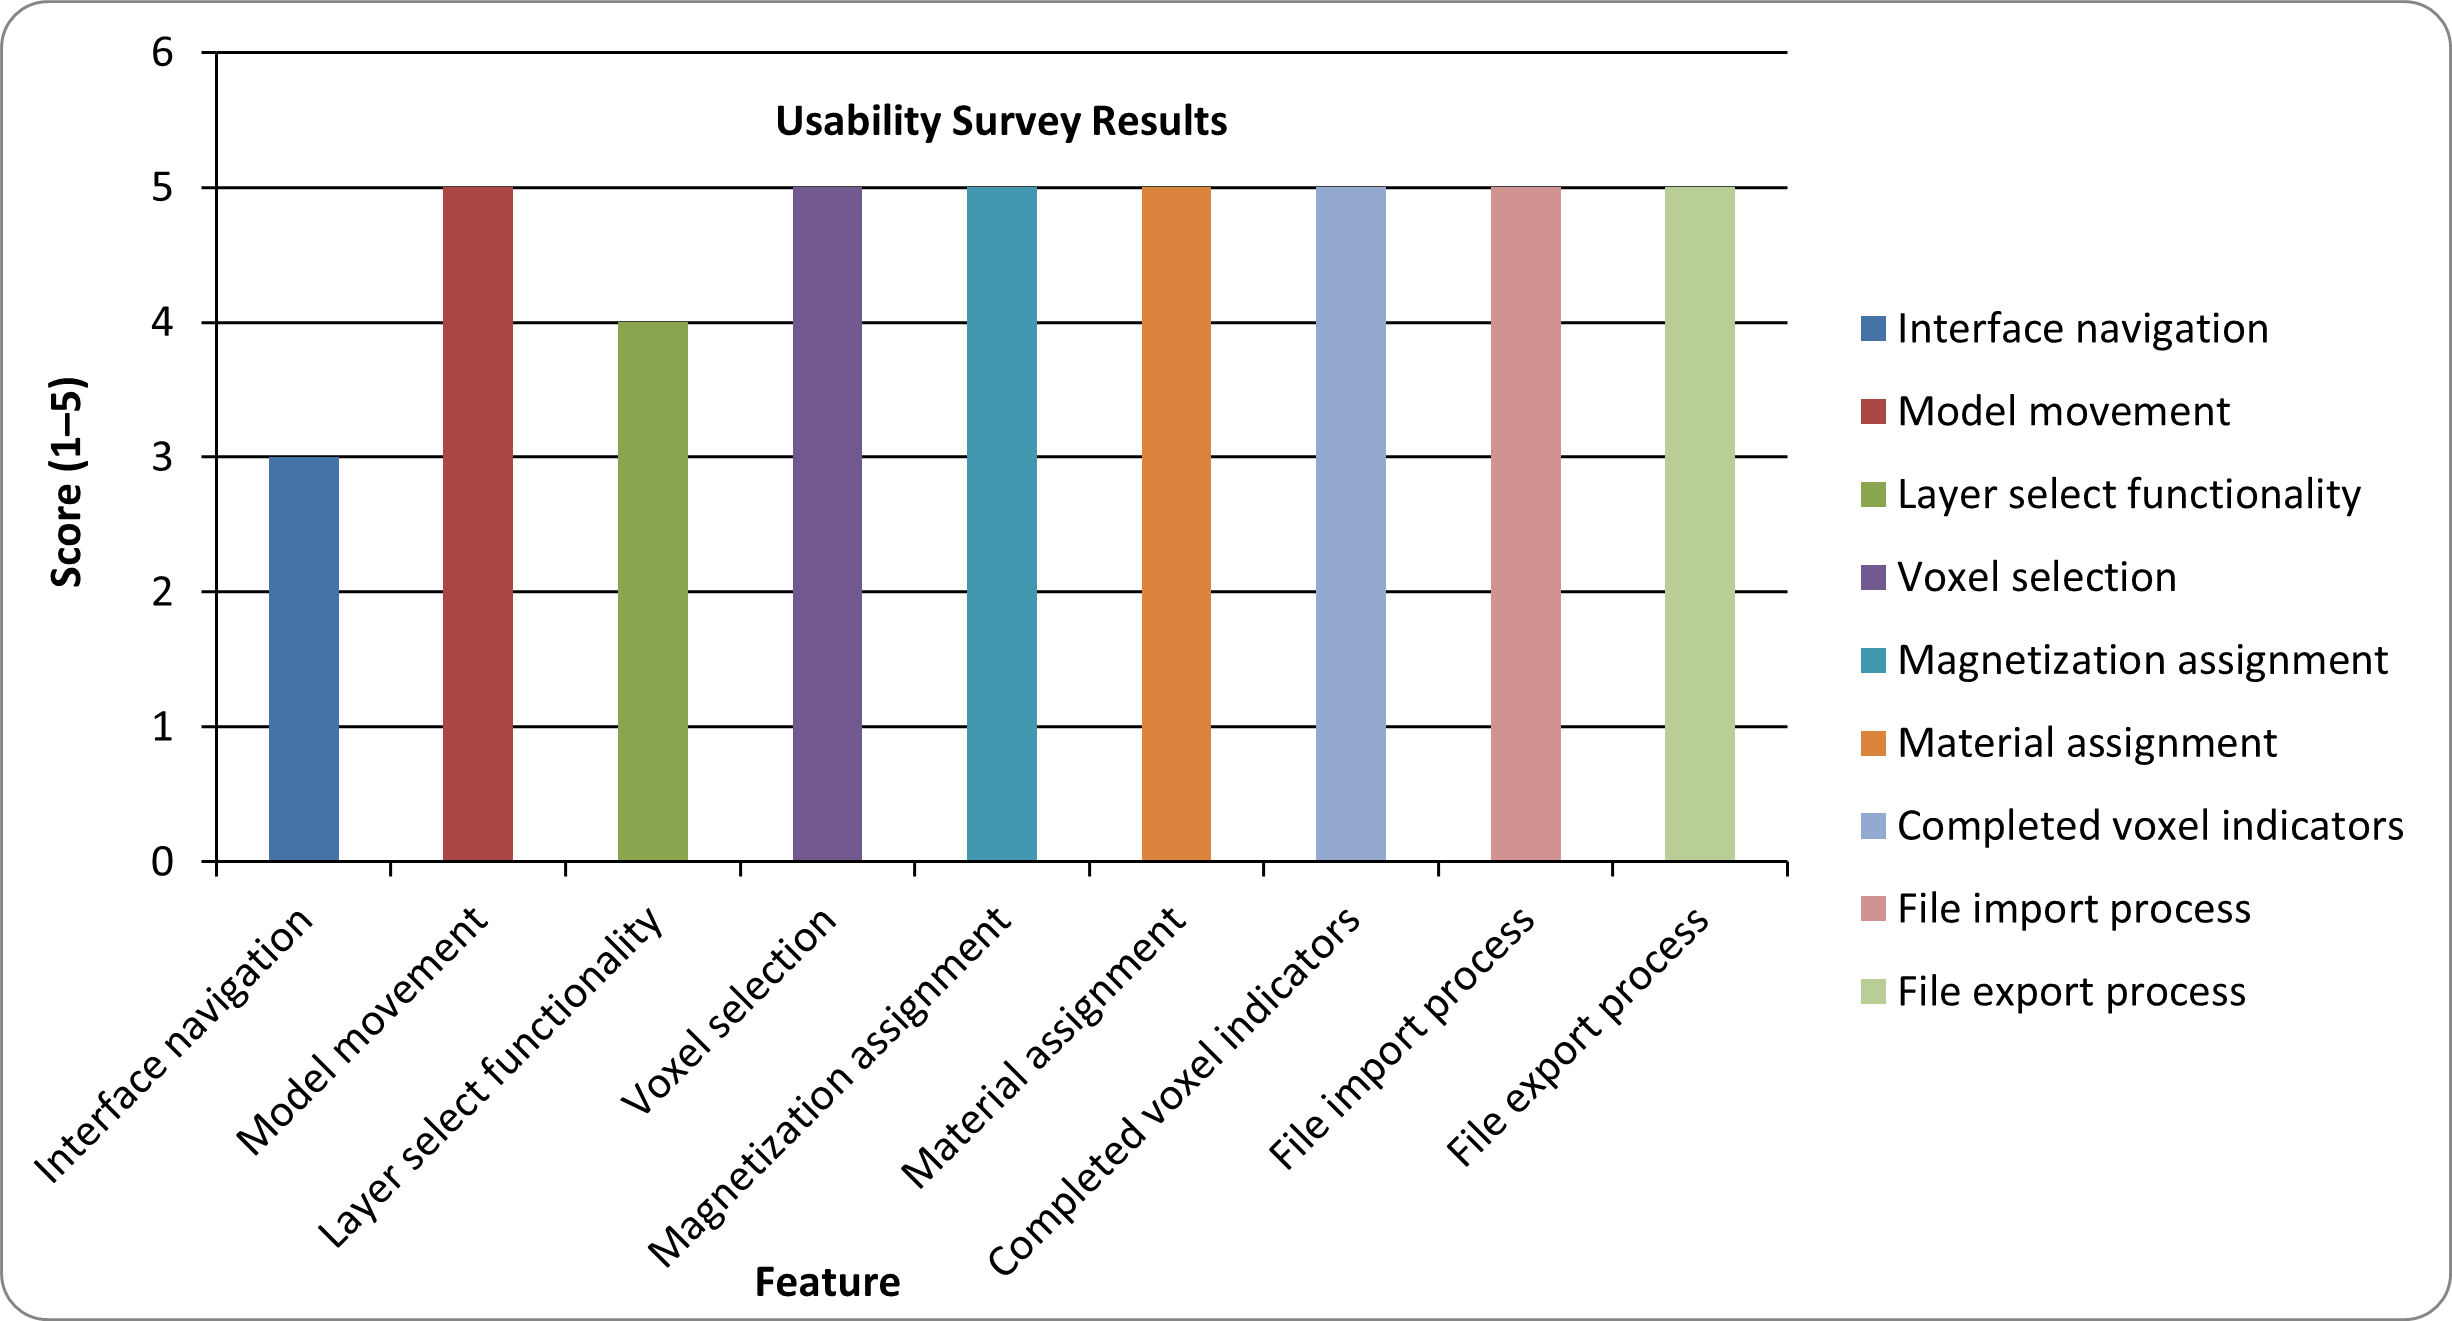
\includegraphics[width=0.8\textwidth]{images/usability_chart.png}
\caption{User Usability Survey Results}
\end{figure}

\subsubsection{Discussion}

The usability evaluation indicated that users generally found the voxel editing system intuitive and effective for performing the primary workflow tasks. Participants reported that the main system features were easy to understand and operate, particularly the voxel editing tools available in the layer editor.

One feature that was specifically highlighted by users was the lasso selection tool for voxels within the layer editor, which allowed users to efficiently select groups of voxels for editing. Participants also appreciated the ability to assign colors to materials, as the color-coded materials made it easier to visually identify different voxel regions within both the layer editor and the model viewer.

Users also indicated that the overall workflow of the application was intuitive. Core operations such as importing STL files, exporting models, editing voxels, and viewing partitions were generally performed without difficulty.

The only stage that presented some challenges for users was the process of loading previously voxelized files. This process includes an additional interaction step compared to other tasks, which increased its perceived complexity. However, users were still able to complete the operation successfully after understanding the workflow.

Overall, the results suggest that the interface design and editing workflow support efficient interaction with the voxel editing system while still leaving room for minor usability improvements.

\subsubsection{Feedback and Implementation Plan}

User feedback collected during the usability evaluation provided several suggestions for improving the usability and workflow of the voxel editing system. The feedback and the planned implementation actions are summarized in Table~\ref{tab:usability-feedback}.

\begin{table}[H]
\centering
\caption{Usability Feedback and Implementation Plan}
\label{tab:usability-feedback}
\begin{tabular}{|p{4cm}|p{6cm}|p{6cm}|}
\hline
\textbf{Feedback Area} & \textbf{User Feedback} & \textbf{Implementation Plan} \\ \hline

Magnetization Visualization & Users suggested adding a visual indicator (such as an ``X'') on voxels whose magnetization has been modified from the default value. & This feature will be implemented by adding a marker on edited voxels in the layer editor to improve visibility of magnetization changes. \\ \hline

Voxelized File Loading & Some users found the process of opening and loading voxelized files slightly more complex due to the additional interaction step required. & No immediate change is planned as the functionality is complete and operates correctly, but documentation may be improved to clarify the workflow. \\ \hline

Partition Viewing & Users suggested that partitions should not always be centered automatically when viewed. & This suggestion will be evaluated and adjusted to the viewing behaviour in next revision. \\ \hline

Layer Viewing Orientation & Some participants suggested that viewing layers from a top-to-bottom orientation may be more intuitive than the current right-to-left presentation. & This suggestion will be investigated to determine whether alternative viewing modes can be supported. \\ \hline

Saving Behaviour & Users requested the ability to overwrite files when saving using the same name. & A file overwrite confirmation option may be added in future updates. \\ \hline

Partition Management & Users suggested the ability to rename partitions after they are created. & This feature will be evaluated and added in future development iterations. \\ \hline

\end{tabular}
\end{table}
\subsection{Performance}

\subsubsection{Methodology}

Performance testing was conducted according to the procedures defined in the VnV Plan, specifically tests \texttt{test-PS-1} (Scalability Validation), \texttt{test-PS-2} (Operational Performance Validation), and \texttt{test-PS-3} (Resource Usage Validation). A set of STL models of varying sizes was used to evaluate system scalability, operational latency, and resource usage. The tests measured the time required for importing models, visualizing voxel structures, performing editing operations, and exporting completed models. Additionally, CPU and GPU usage were monitored while executing core operations. 

\subsubsection{Results}

The scalability test evaluated the relationship between model size and import time. Five STL files with increasing voxel counts were imported sequentially and the time required to complete the import process was recorded. All resulting voxel models rendered correctly within the application.

\begin{table}[H]
\centering
\caption{Scalability Test Results}
\begin{tabular}{|c|c|c|}
\hline
\textbf{File} & \textbf{Estimated Voxels} & \textbf{Import Time (s)} \\
\hline
F1 & 120 & 0.8 \\
F2 & 900 & 1.1 \\
F3 & 4500 & 1.9 \\
F4 & 18000 & 3.4 \\
F5 & 42000 & 5.2 \\
\hline
\end{tabular}
\end{table}

The relationship between voxel count and import time is illustrated in Figure~\ref{fig:import_scalability}.

\begin{figure}[H]
\centering
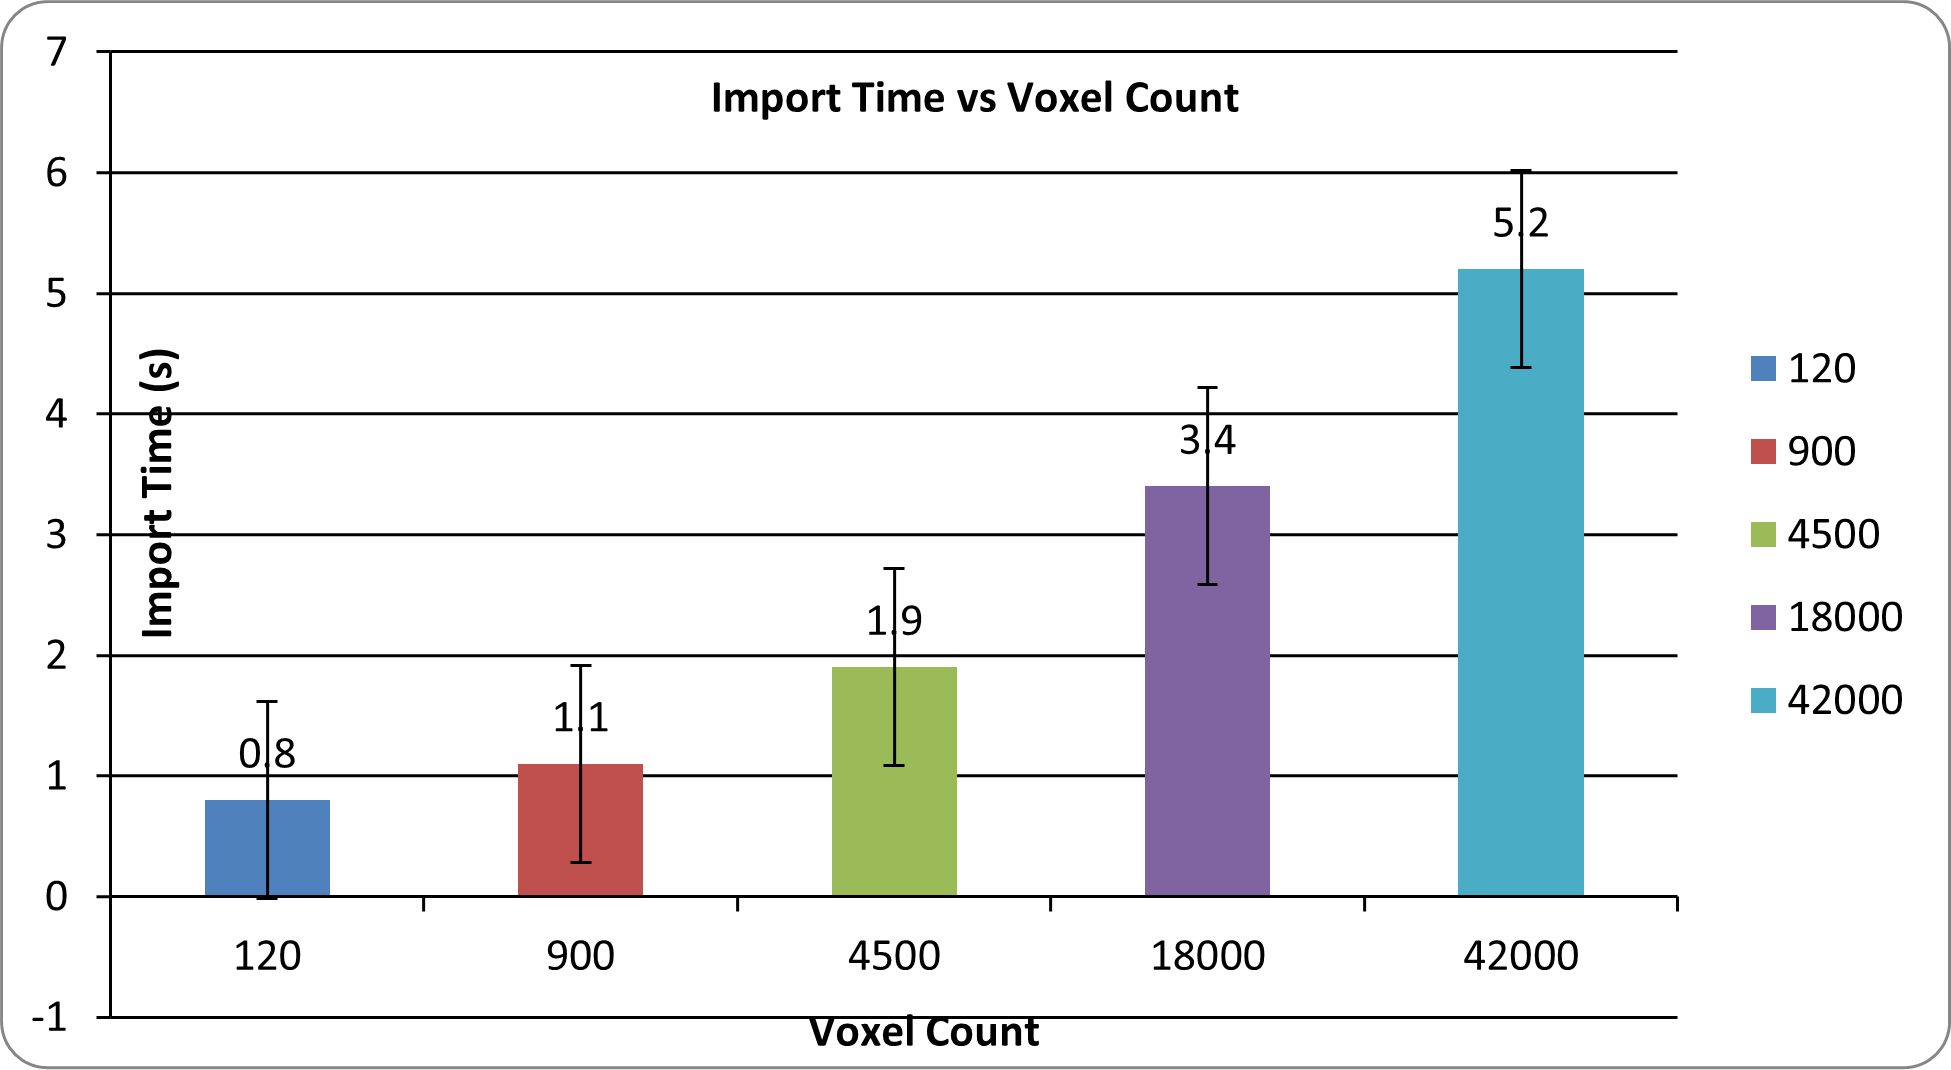
\includegraphics[width=0.8\textwidth]{images/import_scalability.png}
\caption{Import Time vs Voxel Count}
\label{fig:import_scalability}
\end{figure}

User interaction counts were measured for core system actions including model import, viewing operations, voxel editing, and export.
\begin{table}[H]
\centering
\caption{Operation Latency Results}
\begin{tabular}{|c|c|}
\hline
\textbf{Operation} & \textbf{Interactions} \\
\hline
Import Model & 3 \\
Rotate Model & 2 \\
Open Layer View & 4 \\
Edit Single Voxel & 5 \\
Edit 100 Voxels & 5 \\
Edit Full Layer & 5 \\
Export Project & 3 \\
\hline
\end{tabular}
\end{table}

The latency for the various operations is visualized in Figure~\ref{fig:operation_latency}.

\begin{figure}[H]
\centering
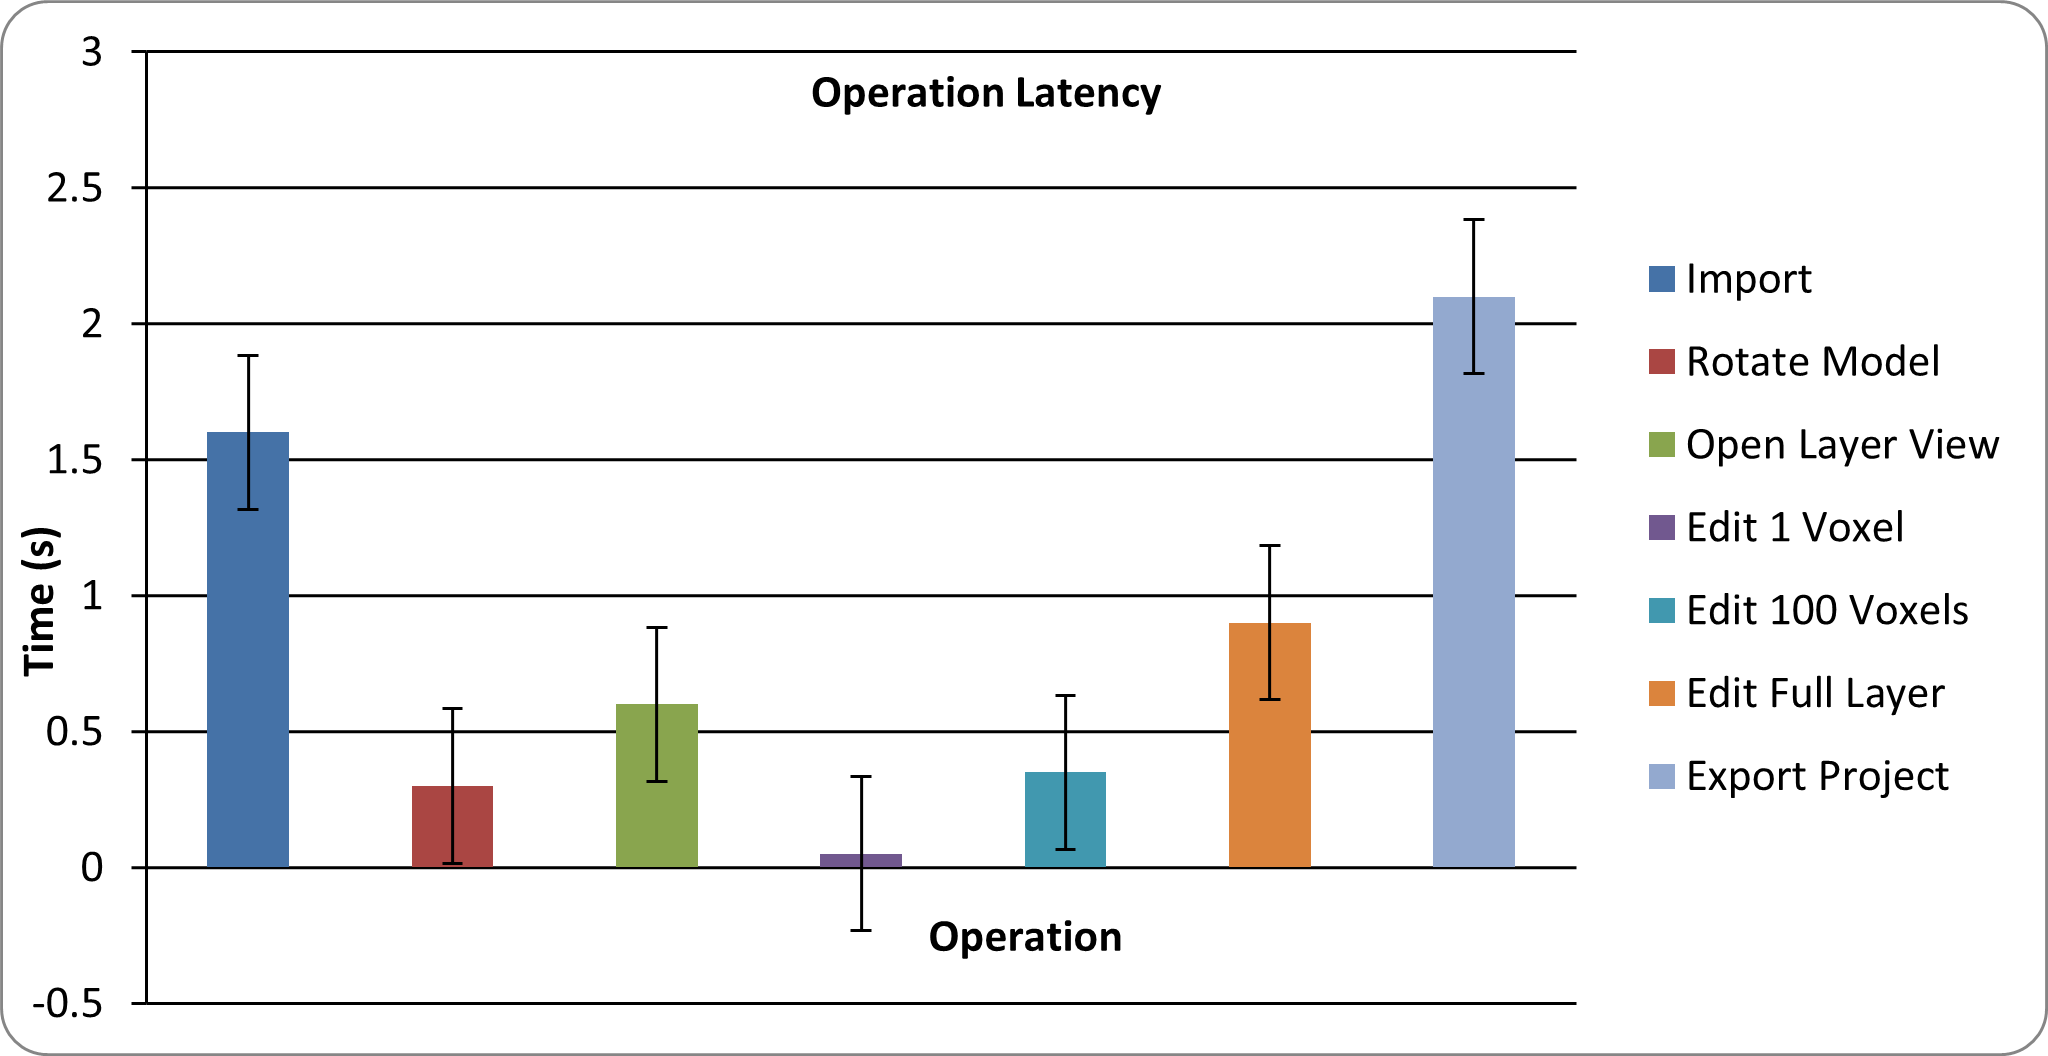
\includegraphics[width=0.8\textwidth]{images/operation_latency.png}
\caption{Operation Latency Measurements}
\label{fig:operation_latency}
\end{figure}

Resource usage during testing remained within acceptable limits. CPU usage ranged between 18--32\%, while GPU usage ranged between 6--14\% during voxel processing and visualization.

\subsubsection{Discussion}

The results demonstrate that the system scales appropriately with increasing voxel counts while maintaining acceptable performance. Import times increased gradually as model size grew, indicating that the voxelization and visualization pipeline handles larger models efficiently.

Core editing operations such as voxel selection and modification were executed with minimal latency, allowing users to interact with the voxel editor without noticeable delay. Export operations required slightly more processing time due to file writing and data serialization but remained within acceptable limits.

Overall, the results confirm that the system satisfies the performance requirements defined in the VnV plan, demonstrating stable operation, scalable processing behaviour, and acceptable hardware resource usage across a range of model sizes.
\subsection{Compliance}

\subsubsection{Methodology}

Compliance testing was performed according to the procedures defined in the VnV plan (tests \texttt{test-CO-1} through \texttt{test-CO-4}). The evaluation focused on verifying operating system compatibility, file import and export compatibility, project file reliability during unexpected interruptions, and adherence to coding standards.

Compliance testing followed the procedures defined in the VnV Plan through tests \texttt{test-CO-1} to \texttt{test-CO-4}, covering operating system compatibility, file compatibility, project file fail-safe behaviour, and PEP8 coding standard compliance.

\subsubsection{Results}

The Windows and Linux compatibility test confirmed that the application could be successfully installed and executed on both operating systems. After installation, the application was opened and core functionalities such as importing STL files, editing voxel structures, and exporting project files were successfully performed on both platforms.

Import and export compatibility was verified by importing CAD models into the system, performing voxel editing operations, and exporting the resulting files to the 3D-printer ready format. The exported files were inspected and confirmed to be correctly formatted and complete.

The project file fail-safe test was conducted by intentionally interrupting the export process while a project file was being written. After restarting the application, the original project file was compared with a backup copy. No differences were observed, confirming that the project file remained unaltered.

Finally, static analysis was conducted on the codebase using a linting tool to verify compliance with the PEP8 coding standard. Minor formatting warnings were addressed during development, and the final codebase was verified to conform to the required style guidelines.

\subsubsection{Discussion}

The compliance tests demonstrate that the application satisfies the compatibility and reliability requirements defined in the VnV plan. The system operates correctly across supported operating systems, maintains file integrity during unexpected interruptions, and adheres to recognized Python coding standards. These results confirm that the system meets the specified compliance requirements.

\subsection{Maintainability}

\subsubsection{Methodology}

Maintainability was evaluated through manual review of the application codebase and associated documentation as described in test MA-1 of the VnV plan. The evaluation focused on modularity of the code structure, quality of documentation, clarity of naming conventions, and readability of comments within the code.

\subsubsection{Results}

The codebase was reviewed to ensure that system components were separated into well-defined modules responsible for specific aspects of the application, including voxel editing, visualization, file management, and user interface functionality. This modular architecture allows developers to modify individual components without requiring extensive changes across the entire system.

Function and class definitions were reviewed to ensure that appropriate comments and documentation were provided. Complex operations and algorithms include explanatory comments to improve readability and maintainability. Naming conventions for functions, classes, and variables were found to be consistent and descriptive.

Associated documentation describing the system architecture and functionality was also reviewed and determined to be sufficiently detailed and readable for future developers.

\subsubsection{Discussion}

The maintainability evaluation confirms that the application codebase is organized in a modular and well-documented manner. The use of clear naming conventions, explanatory comments, and structured documentation supports future development and maintenance activities. As a result, the system satisfies the maintainability requirements defined in the VnV plan.

\subsection{Security}

Security requirements defined in the Hazard Analysis document were not tested independently as standalone tests. Instead, they were implicitly verified through existing functional and unit tests across multiple system components.

Several security-related constraints were validated through tests that verify correct system behavior under edge conditions. For example, editing and visualization managers include unit tests that ensure voxel selection limits are enforced and that operations remain within defined memory and performance constraints.

Other security-related requirements are implicitly verified through import and export validation tests, which ensure that file handling operations do not produce corrupted outputs or unintended system states.

Some security constraints related to hardware limitations could not be tested directly due to the absence of specialized hardware environments. These constraints were instead verified through unit tests that simulate reduced system resources.

Overall, the existing functional and unit testing framework provides coverage for the security requirements defined in the Hazard Analysis document, ensuring that the system operates safely within expected constraints.

	
\section{Comparison to Existing Implementation}\label{sec:comparison}

\progname\ serves as an alternative to commercial multiphysics tools such as \href{https://www.comsol.com/}{COMSOL Multiphysics\textregistered} for workflows that involve editing and configuring voxel-based or mesh-based models. In the lab setting, \progname\ addresses several pain points that research assistants experience when using COMSOL for similar tasks.

COMSOL is a full-featured simulation platform, but manual editing across many voxels is tedious and error-prone. Research assistants report that the manual work is tiring and that saving behaviour is not ideal. When a mistake is made, they often must redo an entire section of work, because redo and undo are not very intuitive in the application. In addition, crashes occur frequently, and COMSOL does not offer saved backups on a server, so recovery after a crash can mean lost work.

\progname\ is designed to improve this workflow by providing clearer redo and undo behaviour and by supporting bulk actions across many voxels. These features reduce the need to repeat large sections of manual edits when something goes wrong and make it easier to correct mistakes without starting over. The combination of intuitive undo/redo and server-backed or local project saving (where implemented) aims to make \progname\ a more forgiving and efficient tool for repetitive voxel-level editing in the research lab.

\section{Unit Testing}\label{sec:unit-testing}

This section reports \textbf{test results} and evidence for the system unit tests. The emphasis is on outcomes and evidence, not on the rationale for test selection (see the \href{https://github.com/OmarHassanAdelhamid/Five-of-a-Kind-capstone-project-/blob/main/docs/VnVPlan/VnVPlan.pdf}{VnV Plan} for that). Test cases are organized by manager: Import Manager (TC1--TC5), Visualization Manager (TC4--TC11), Editing Manager (TC12--TC61), and Export Manager (TC62--TC69).

For each test case, the tables below provide: \textbf{test case name} (TC id), \textbf{initial state} (implied by the Ref.\ Req.\ and test context), \textbf{input} (Action), \textbf{expected result}, and \textbf{whether actual output matched expected} (Result: Pass/Fail). Actual outcomes are backed by automated test runs; see Section~\ref{sec:automated-testing} for how to reproduce.

\subsection{Import Manager Tests}
\newcounter{testcase}
\newcommand{\testcount}{\stepcounter{testcase}\thetestcase}
\renewcommand{\arraystretch}{1.2}

\subsubsection{CAD File Import and Project Management}
Table~\ref{table:im_cad_tests} gives the results for STL file import and project management tests (TC1--TC5).

\begin{longtable}{c
    >{\raggedright\arraybackslash}p{1.5cm}
    >{\raggedright\arraybackslash}p{4.2cm}
    >{\raggedright\arraybackslash}p{3.5cm}
  >{\raggedright\arraybackslash}p{2.5cm} c}
  \caption{Import Manager: STL File Import and Project Management Test Cases}
  \label{table:im_cad_tests} \\
  \toprule
  \textbf{TC} & \textbf{Ref. Req.} & \textbf{Action} &
  \textbf{Expected Result} & \textbf{Actual Result} & \textbf{Result} \\
  \midrule
  \endfirsthead

  \multicolumn{6}{l}{\textit{(Continued from previous page)}} \\
  \toprule
  \textbf{TC} & \textbf{Ref. Req.} & \textbf{Action} &
  \textbf{Expected Result} & \textbf{Actual Result} & \textbf{Result} \\
  \midrule
  \endhead

  \multicolumn{6}{r}{\textit{Continued on next page}} \\
  \endfoot

  \bottomrule
  \endlastfoot

  TC1 & F211 & Provide a valid STL file to system through file settings panel & STL file is uploaded successfully to the system, and saved to the sample file directory & All assertions are met and passed by backend unit test & \cellcolor{green} Pass \\ \midrule
  TC2 & F211 & Browse all uploaded STL files in the sample file directory & System displays a list of all uploaded STL files in the sample file directory & All assertions are met and passed by backend unit test & \cellcolor{green} Pass \\ \midrule
  TC3 & F211 & Browse all uploaded STL files, without ever uploading a STL file & System displays an empty list of uploaded STL files & All assertions are met and passed by backend unit test & \cellcolor{green} Pass \\ \midrule
  TC4 & F211 & Provide a file with unsupported format (e.g.\ .txt, .jpg, .pdf) to system through file settings panel & System rejects the file and displays an error indicating unsupported format & All assertions are met and passed by backend unit test & \cellcolor{green} Pass \\ \midrule
  TC5 & F212 & Open a previously uploaded STL file & System loads the STL file from the sample file directory & All assertions are met and passed by backend unit test & \cellcolor{green} Pass \\
\end{longtable}

\subsubsection{Model Configuration and Slicing}
Table~\ref{table:im_config_tests} gives the results for model configuration and slicing tests (TC6--TC12).

\begin{longtable}{c
    >{\raggedright\arraybackslash}p{1.5cm}
    >{\raggedright\arraybackslash}p{4.2cm}
    >{\raggedright\arraybackslash}p{3.5cm}
  >{\raggedright\arraybackslash}p{2.5cm} c}
  \caption{Import Manager: Model Configuration and Slicing Test Cases}
  \label{table:im_config_tests} \\
  \toprule
  \textbf{TC} & \textbf{Ref. Req.} & \textbf{Action} &
  \textbf{Expected Result} & \textbf{Actual Result} & \textbf{Result} \\
  \midrule
  \endfirsthead

  \multicolumn{6}{l}{\textit{(Continued from previous page)}} \\
  \toprule
  \textbf{TC} & \textbf{Ref. Req.} & \textbf{Action} &
  \textbf{Expected Result} & \textbf{Actual Result} & \textbf{Result} \\
  \midrule
  \endhead

  \multicolumn{6}{r}{\textit{Continued on next page}} \\
  \endfoot

  \bottomrule
  \endlastfoot

  TC6 & F213 & Specify custom voxel size & System applies the dimensions and slices the model into voxels of the requested size & All assertions are met and passed by backend unit test & \cellcolor{green} Pass \\ \midrule
  TC7 & F214 & Specify custom geometric model size & System scales the model to desired model size before slicing & All assertions are met and passed by backend unit test & \cellcolor{green} Pass \\ \midrule
  TC8 & F216 & Import a model containing more than MAX\_VOXELS voxels. & System partitions the model into display sections not exceeding MAX\_VOXELS & All assertions are met and passed by backend unit test & \cellcolor{green} Pass \\ \midrule
  TC9 & F216 & Import a model containing less than MAX\_VOXELS voxels & System returns only one partition with all voxels visible& All assertions are met and passed by backend unit test & \cellcolor{green} Pass \\ \midrule
  TC10 & F216 & Delete a partition with no voxels & System deletes the partition and returns the model to the previous state & All assertions are met and passed by backend unit test & \cellcolor{green} Pass \\ \midrule
  TC11 & F213, F214, F215 & Voxelize uploaded STL model into voxels& System voxelizes the model into voxels of the requested size using Triangle Meshes & All assertions are met and passed by backend unit test & \cellcolor{green} Pass \\ \midrule
  TC12 & F213, F214, F215 & Voxelize non-existing STL model into voxels& System returns an error indicating the STL model does not exist & All assertions are met and passed by backend unit test & \cellcolor{green} Pass \\
\end{longtable}

\subsection{Visualization Manager Tests}

\subsubsection{3D Model Rendering and Display}
Table~\ref{table:vm_rendering_tests} gives the results for 3D model rendering and display tests (TC13--TC16).

\begin{longtable}{c
    >{\raggedright\arraybackslash}p{1.5cm}
    >{\raggedright\arraybackslash}p{4.2cm}
    >{\raggedright\arraybackslash}p{3.5cm}
  >{\raggedright\arraybackslash}p{2.5cm} c}
  \caption{Visualization Manager: 3D Model Rendering and Display Test Cases}
  \label{table:vm_rendering_tests} \\
  \toprule
  \textbf{TC} & \textbf{Ref. Req.} & \textbf{Action} &
  \textbf{Expected Result} & \textbf{Actual Result} & \textbf{Result} \\
  \midrule
  \endfirsthead

  \multicolumn{6}{l}{\textit{(Continued from previous page)}} \\
  \toprule
  \textbf{TC} & \textbf{Ref. Req.} & \textbf{Action} &
  \textbf{Expected Result} & \textbf{Actual Result} & \textbf{Result} \\
  \midrule
  \endhead

  \multicolumn{6}{r}{\textit{Continued on next page}} \\
  \endfoot

  \bottomrule
  \endlastfoot

  TC13 & F221 & Import a STL model into the system & System renders a non-voxelized 3D STL model using Three.js & All assertions are met and passed by frontend unit test & \cellcolor{green} Pass \\ \midrule
  TC14 & F221 & Open a voxelized project from file directory & System renders a voxelized 3D model using Three.js broken down into layers & All assertions are met and passed by frontend unit test & \cellcolor{green} Pass \\ \midrule
  TC15 & F222 & Open a voxelized project from file directory where the number of voxels is greater than MAX\_VOXELS & System displays a partitions panel with more than 1 partition & All assertions are met and passed by frontend unit test & \cellcolor{green} Pass \\ \midrule
  TC16 & F222 & Open a voxelized project from file directory where the number of voxels is less than MAX\_VOXELS & System displays a partitions panel with only 1 partition & All assertions are met and passed by frontend unit test & \cellcolor{green} Pass \\

\end{longtable}

\subsubsection{Layer Focus and Voxel Selection Tests}
Table~\ref{table:vm_layer_tests} gives the results for layer focus and voxel selection tests (TC17--TC24).

\begin{longtable}{c
    >{\raggedright\arraybackslash}p{1.5cm}
    >{\raggedright\arraybackslash}p{4.2cm}
    >{\raggedright\arraybackslash}p{3.5cm}
  >{\raggedright\arraybackslash}p{2.5cm} c}
  \caption{Visualization Manager: Layer Focus and Voxel Selection Test Cases}
  \label{table:vm_layer_tests} \\
  \toprule
  \textbf{TC} & \textbf{Ref. Req.} & \textbf{Action} &
  \textbf{Expected Result} & \textbf{Actual Result} & \textbf{Result} \\
  \midrule
  \endfirsthead

  \multicolumn{6}{l}{\textit{(Continued from previous page)}} \\
  \toprule
  \textbf{TC} & \textbf{Ref. Req.} & \textbf{Action} &
  \textbf{Expected Result} & \textbf{Actual Result} & \textbf{Result} \\
  \midrule
  \endhead

  \multicolumn{6}{r}{\textit{Continued on next page}} \\
  \endfoot

  \bottomrule
  \endlastfoot

  TC17 & F222 & Pick a specific partition to focus on from the partitions panel. & The selected partition is isolated and displayed as a 3D view without any other partitions. & All assertions are met and passed by frontend unit test & \cellcolor{green} Pass \\ \midrule
  TC18 & F223 & Rotate the model using interface controls. & Model rotates smoothly and intuitively & All assertions are met and passed by frontend unit test & \cellcolor{green} Pass \\ \midrule
  TC19 & F223 & Zoom the model using interface controls. & Model zooms smoothly and intuitively & All assertions are met and passed by frontend unit test & \cellcolor{green} Pass \\ \midrule
  TC20 & F224 & Select a specific layer to focus on from the 3D model display. & Selected layer is isolated, layer editor is opened displaying the layer voxels and properties in a 2D view. & All assertions are met and passed by frontend unit test & \cellcolor{green} Pass \\ \midrule
  TC21 & F225 & Select individual voxel within the focused layer from the layer editor. & The selected voxel is highlighted in the 2D layer view & All assertions are met and passed by frontend unit test & \cellcolor{green} Pass \\ \midrule
  TC22 & F225 & Select multiple voxels within the focused layer from the layer editor using lasso selection. & The selected voxels are highlighted in the 2D layer view & All assertions are met and passed by frontend unit test & \cellcolor{green} Pass \\ \midrule
  TC23 & F225 & Select all voxels in the partition on the 3D view (CTRL+A) & All voxels in the partition are highlighted in the 3D view & All assertions are met and passed by frontend unit test & \cellcolor{green} Pass \\ \midrule
  TC24 & F225 & Select all voxels in the layer on the 2D layer view (CTRL+A) & All voxels in the layer are highlighted in the 2D layer view & All assertions are met and passed by frontend unit test & \cellcolor{green} Pass \\
\end{longtable}

\subsubsection{Material and Magnetization Tracking}
Table~\ref{table:vm_tracking_tests} gives the results for material and magnetization tracking tests (TC25--TC26).

\begin{longtable}{c
    >{\raggedright\arraybackslash}p{1.5cm}
    >{\raggedright\arraybackslash}p{4.2cm}
    >{\raggedright\arraybackslash}p{3.5cm}
  >{\raggedright\arraybackslash}p{2.5cm} c}
  \caption{Visualization Manager: Material and Magnetization Tracking Test Cases}
  \label{table:vm_tracking_tests} \\
  \toprule
  \textbf{TC} & \textbf{Ref. Req.} & \textbf{Action} &
  \textbf{Expected Result} & \textbf{Actual Result} & \textbf{Result} \\
  \midrule
  \endfirsthead

  \multicolumn{6}{l}{\textit{(Continued from previous page)}} \\
  \toprule
  \textbf{TC} & \textbf{Ref. Req.} & \textbf{Action} &
  \textbf{Expected Result} & \textbf{Actual Result} & \textbf{Result} \\
  \midrule
  \endhead

  \multicolumn{6}{r}{\textit{Continued on next page}} \\
  \endfoot

  \bottomrule
  \endlastfoot

  TC25 & F226 & Assign material IDs to a voxel or multiple voxels in the layer editor. & The color of the voxels are updated to the assigned material color. & All assertions are met and passed by frontend unit test & \cellcolor{green} Pass \\ \midrule
  TC26 & F227 & Assign magnetization to a voxel or multiple voxels in the layer editor. & The voxels assigned will be highlighted with a X-arrow icon indicating magnetization. & All assertions are met and passed by frontend unit test & \cellcolor{green} Pass \\

\end{longtable}

\subsection{Editing Manager Tests}
The Editing Manager tests are organized into three subsections: editing a voxel (TC27--TC49), utilizing the history manager (TC50--TC58), and saving project (TC59--TC62).

\subsubsection{Editing a voxel}
Table~\ref{table:em_voxel_tests} gives the results for voxel editing tests (TC27--TC49): magnetization and material assignment, layer access, and adding, deleting, or resetting voxels.

\begin{longtable}{c
    >{\raggedright\arraybackslash}p{1.5cm}
    >{\raggedright\arraybackslash}p{3.8cm}
    >{\raggedright\arraybackslash}p{3.5cm}
  >{\raggedright\arraybackslash}p{2.2cm} c}
  \caption{Editing Manager: Editing a voxel (system and backend)}
  \label{table:em_voxel_tests} \\
  \toprule
  \textbf{TC} & \textbf{Ref. Req.} & \textbf{Action} &
  \textbf{Expected Result} & \textbf{Actual Result} & \textbf{Result} \\
  \midrule
  \endfirsthead

  \multicolumn{6}{l}{\textit{(Continued from previous page)}} \\
  \toprule
  \textbf{TC} & \textbf{Ref. Req.} & \textbf{Action} &
  \textbf{Expected Result} & \textbf{Actual Result} & \textbf{Result} \\
  \midrule
  \endhead

  \multicolumn{6}{r}{\textit{Continued on next page}} \\
  \endfoot

  \bottomrule
  \endlastfoot

  TC27 & F231 & Update magnetization of a single voxel (e.g.\ x=1.0, y=0.0, z=0.0). & System saves the magnetization vector of the voxel to the database & All assertions are met and passed by backend unit test & \cellcolor{green} Pass \\ \midrule
  TC28 & F231 & Update magnetization of a multiple voxels (e.g.\ x=1.0, y=0.0, z=0.0). & System saves the magnetization vector of the voxels to the database & All assertions are met and passed by backend unit test & \cellcolor{green} Pass \\ \midrule
  TC29 & F231 & Update magnetization of a non-existing voxel (e.g.\ x=1.0, y=0.0, z=0.0). & System returns an error indicating the voxel does not exist & All assertions are met and passed by backend unit test & \cellcolor{green} Pass \\ \midrule
  TC30 & F231 & Update magnetization of a voxel with invalid magnetization vector (e.g.\ x=1.0, y=0.0, z=0.0). & System returns an error indicating the magnetization vector is invalid & All assertions are met and passed by backend unit test & \cellcolor{green} Pass \\ \midrule
  TC31 & F232 & Create a favourite magnetization vector (e.g.\ x=1.0, y=0.0, z=0.0). & System saves the magnetization vector to the favourite bar & All assertions are met and passed by backend unit test & \cellcolor{green} Pass \\ \midrule
  TC32 & F233 & Assign material ID to a single voxel (e.g.\ 2). & System saves the material ID to the voxel and in the database & All assertions are met and passed by backend unit test & \cellcolor{green} Pass \\ \midrule
  TC33 & F233 & Assign material ID to a multiple voxels (e.g.\ 2). & System saves the material ID to the voxels and in the database & All assertions are met and passed by backend unit test & \cellcolor{green} Pass \\ \midrule
  TC34 & F233 & Assign material ID to a non-existing voxel (e.g.\ 2). & System returns an error indicating the voxel does not exist & All assertions are met and passed by backend unit test & \cellcolor{green} Pass \\ \midrule 
  TC35 & F231, F233 & Assign material ID to a voxel and magnetization to a voxel (e.g.\ 2, x=1.0, y=0.0, z=0.0). & System saves the material ID and magnetization vector to the voxel and in the database & All assertions are met and passed by backend unit test & \cellcolor{green} Pass \\ \midrule
  TC36 & F234 & Assign label ``Steel'' to material ID 1. & Material ID 1 is associated with the label ``Steel'' in the database. & All assertions are met and passed by backend unit test & \cellcolor{green} Pass \\ \midrule
  TC37 & F235 & Copy assigned properties from one layer to another layer. & Target layer voxels receive the same material and magnetization properties as the source. & All assertions are met and passed by backend and frontend unit test & \cellcolor{green} Pass \\ \midrule 
  TC38 & F238 & Get list of layers in the project. & The list of layers is returned. & All assertions are met and passed by backend unit test & \cellcolor{green} Pass \\ \midrule
  TC39 & F238 & Get specific layer in the project based on the layer index and axis. & The specific layer is returned. & All assertions are met and passed by backend unit test & \cellcolor{green} Pass \\ \midrule
  TC40 & F238 & Get specific layer with non-existing layer index. & System returns an error indicating the layer index does not exist. & All assertions are met and passed by backend unit test & \cellcolor{green} Pass \\ \midrule
  TC41 & F238 & Get specific layer with non-existing axis. & System returns an error indicating the axis does not exist. & All assertions are met and passed by backend unit test & \cellcolor{green} Pass \\ \midrule
  TC42 & F238 & Get specific layer with non-existing project. & System returns an error indicating the project does not exist. & All assertions are met and passed by backend unit test & \cellcolor{green} Pass \\ \midrule
  TC43 & F238 & Get specific layer with non-existing partition. & System returns an error indicating the partition does not exist. & All assertions are met and passed by backend unit test & \cellcolor{green} Pass \\ \midrule
  TC44 & F239 & Add a new voxel at new indices. & A new voxel is added to the database at the new indices with default material and magnetization. & All assertions are met and passed by backend and frontend unit test & \cellcolor{green} Pass \\ \midrule
  TC45 & F239 & Delete an existing voxel. & A voxel is removed from the database at the existing indices. & All assertions are met and passed by backend and frontend unit test & \cellcolor{green} Pass \\ \midrule
  TC46 & F239 & Delete a non-existent voxel. & System returns an error indicating the voxel does not exist. & All assertions are met and passed by backend unit test & \cellcolor{green} Pass \\ \midrule
  TC47 & F2310 & Reset materials on selected voxels. & The voxels are reset to the default material in the database. & All assertions are met and passed by backend and frontend unit test & \cellcolor{green} Pass \\ \midrule
  TC48 & F2310 & Reset magnetizations on selected voxels. & The voxels are reset to the default magnetization in the database. & All assertions are met and passed by backend and frontend unit test & \cellcolor{green} Pass \\ \midrule
  TC49 & F2310 & Reset materials and magnetizations on selected voxels. & The voxels are reset to the default material and magnetization in the database. & All assertions are met and passed by backend and frontend unit test & \cellcolor{green} Pass \\
\end{longtable}

\subsubsection{Utilizing the history manager}
Table~\ref{table:em_history_tests} gives the results for history manager tests (TC50--TC58): undo, redo, and clear history.

\begin{longtable}{c
    >{\raggedright\arraybackslash}p{1.5cm}
    >{\raggedright\arraybackslash}p{3.8cm}
    >{\raggedright\arraybackslash}p{3.5cm}
  >{\raggedright\arraybackslash}p{2.2cm} c}
  \caption{Editing Manager: Utilizing the history manager (backend)}
  \label{table:em_history_tests} \\
  \toprule
  \textbf{TC} & \textbf{Ref. Req.} & \textbf{Action} &
  \textbf{Expected Result} & \textbf{Actual Result} & \textbf{Result} \\
  \midrule
  \endfirsthead

  \multicolumn{6}{l}{\textit{(Continued from previous page)}} \\
  \toprule
  \textbf{TC} & \textbf{Ref. Req.} & \textbf{Action} &
  \textbf{Expected Result} & \textbf{Actual Result} & \textbf{Result} \\
  \midrule
  \endhead

  \multicolumn{6}{r}{\textit{Continued on next page}} \\
  \endfoot

  \bottomrule
  \endlastfoot

  TC50 & F237 & Undo any updates made to a voxel. & The changes are undone and the voxel returns to the previous state. & All assertions are met and passed by backend unit test & \cellcolor{green} Pass \\ \midrule
  TC51 & F237 & Redo any undone updates to a voxel. & The changes are redone and the voxel returns to the previous state. & All assertions are met and passed by backend unit test & \cellcolor{green} Pass \\ \midrule
  TC52 & F237 & Undo any added voxels. & The voxels are removed from the database. & All assertions are met and passed by backend unit test & \cellcolor{green} Pass \\ \midrule
  TC53 & F237 & Redo any deleted voxels. & The voxels are added back to the database. & All assertions are met and passed by backend unit test & \cellcolor{green} Pass \\ \midrule
  TC54 & F237 & Undo any reset material on a voxel. & The voxel is reset to the default material. & All assertions are met and passed by backend unit test & \cellcolor{green} Pass \\ \midrule
  TC55 & F237 & Redo any reset material on a voxel. & The voxel is reset to the default material. & All assertions are met and passed by backend unit test & \cellcolor{green} Pass \\ \midrule
  TC56 & F237 & Undo when history empty. & System returns an error indicating the history is empty & All assertions are met and passed by backend unit test & \cellcolor{green} Pass \\ \midrule
  TC57 & F237 & Redo when redo stack empty. & System returns an error indicating the redo stack is empty & All assertions are met and passed by backend unit test & \cellcolor{green} Pass \\ \midrule
  TC58 & F237 & Clear history. & Both history and redo stacks empty. & All assertions are met and passed by backend unit test & \cellcolor{green} Pass \\
\end{longtable}

\subsubsection{Saving project}
Table~\ref{table:em_save_tests} gives the results for saving project tests (TC59--TC62).

\begin{longtable}{c
    >{\raggedright\arraybackslash}p{1.5cm}
    >{\raggedright\arraybackslash}p{3.8cm}
    >{\raggedright\arraybackslash}p{3.5cm}
  >{\raggedright\arraybackslash}p{2.2cm} c}
  \caption{Editing Manager: Saving project (backend)}
  \label{table:em_save_tests} \\
  \toprule
  \textbf{TC} & \textbf{Ref. Req.} & \textbf{Action} &
  \textbf{Expected Result} & \textbf{Actual Result} & \textbf{Result} \\
  \midrule
  \endfirsthead

  \multicolumn{6}{l}{\textit{(Continued from previous page)}} \\
  \toprule
  \textbf{TC} & \textbf{Ref. Req.} & \textbf{Action} &
  \textbf{Expected Result} & \textbf{Actual Result} & \textbf{Result} \\
  \midrule
  \endhead

  \multicolumn{6}{r}{\textit{Continued on next page}} \\
  \endfoot

  \bottomrule
  \endlastfoot

  TC59 & F236 & Save the project automatically. & The project is saved to the database. & All assertions are met and passed by backend unit test & \cellcolor{green} Pass \\ \midrule
  TC60 & F2311 & Save the project manually. & The project is saved to the database. & All assertions are met and passed by backend unit test & \cellcolor{green} Pass \\ \midrule
  TC61 & F2311 & Save a non-existent project. & System returns an error indicating the project does not exist. & All assertions are met and passed by backend unit test & \cellcolor{green} Pass \\ \midrule
  TC62 & F2311 & Save a project with invalid data. & System returns an error indicating the project data is invalid. & All assertions are met and passed by backend unit test & \cellcolor{green} Pass \\
\end{longtable}

\subsection{Export Manager Tests}

\subsubsection{Export Validation and File Export}
Table~\ref{table:xm_tests} gives the results for export validation and file export (TC63--TC72).

\begin{longtable}{c
    >{\raggedright\arraybackslash}p{1.8cm}
    >{\raggedright\arraybackslash}p{4.2cm}
    >{\raggedright\arraybackslash}p{4cm}
  >{\raggedright\arraybackslash}p{3cm} c}
  \caption{Export Manager Test Cases}
  \label{table:xm_tests} \\
  \toprule
  \textbf{TC} & \textbf{Ref. Req.} & \textbf{Action} &
  \textbf{Expected Result} & \textbf{Actual Result} & \textbf{Result} \\
  \midrule
  \endfirsthead

  \multicolumn{6}{l}{\textit{(Continued from previous page)}} \\
  \toprule
  \textbf{TC} & \textbf{Ref. Req.} & \textbf{Action} &
  \textbf{Expected Result} & \textbf{Actual Result} & \textbf{Result} \\
  \midrule
  \endhead

  \multicolumn{6}{r}{\textit{Continued on next page}} \\
  \endfoot

  \bottomrule
  \endlastfoot

  TC63 & F241 & Validate all voxels have magnetization. & System checks if all voxels have magnetization and returns an error if any voxels are missing magnetization. & All assertions are met and passed by backend unit test & \cellcolor{green} Pass \\ \midrule
  TC64 & F241 & Validate all voxels have material. & System checks if all voxels have material and returns an error if any voxels are missing material. & All assertions are met and passed by backend unit test & \cellcolor{green} Pass \\ \midrule
  TC65 & F242 & Export CSV file of an existing project. & System exports a CSV file with all voxel metadata. & All assertions are met and passed by backend unit test & \cellcolor{green} Pass \\ \midrule
  TC66 & F242 & Export CSV file of a non-existent project. & System returns an error indicating the project does not exist. & All assertions are met and passed by backend unit test & \cellcolor{green} Pass \\ \midrule
  TC67 & F242 & Export CSV file of a project with invalid data. & System returns an error indicating the project data is invalid. & All assertions are met and passed by backend unit test & \cellcolor{green} Pass \\ \midrule
  TC68 & F243 & Export project file of an existing project. & System exports a project file with all project data. & All assertions are met and passed by backend unit test & \cellcolor{green} Pass \\ \midrule
  TC69 & F243 & Export project file of a non-existent project. & System returns an error indicating the project does not exist. & All assertions are met and passed by backend unit test & \cellcolor{green} Pass \\ \midrule
  TC70 & F243 & Export project file of a project with invalid data. & System returns an error indicating the project data is invalid. & All assertions are met and passed by backend unit test & \cellcolor{green} Pass \\ \midrule
  TC71 & F245 & Export model with summary option enabled. & System exports a model file with a summary of the model. & All assertions are met and passed by backend unit test & \cellcolor{green} Pass \\ \midrule
  TC72 & F241 & Export operation is interrupted (simulated failure). & Original project data remains intact and unaltered. & All assertions are met and passed by backend unit test & \cellcolor{green} Pass \\
\end{longtable}

\section{Changes Due to Testing}
\label{sec:changes-due-to-testing}

During the VnV process, several changes to the project that were made based on the feedback from the stakeholders (supervisor and graduate students) that will be used to improve the system. These changes are related to the usability and user input, interaction flow, and performance adjustments.

\subsection{Usability and User Input Adjustments}

Feedback from usability testing led to the following usability and user-input changes:

\begin{itemize}
  \item \textbf{Project and file menus:} A project popup after selecting a file to show existing projects, improving feedback and selection, as it was not clear where to navigate to open a project.
  \item \textbf{Layer editor:} The magnitude control in the layer editor was removed to reduce clutter and confusion and as it was not used by the stakeholders.
  \item \textbf{File and material naming:} File naming was reviewed to handle spaces and to indicate when a file with the same name already exists. Material naming in settings was reviewed for clarity and consistency.
  \item \textbf{Magnetization display:} A checkmark or toggle was added to show or hide magnetization, giving users control over what is displayed.
  \item \textbf{Partition behaviour:} Default partition centring was changed so partitions are not automatically centred. A rename-partition capability was added.
\end{itemize}

\subsection{Interaction Flow Adjustments}

The following changes address the sequence of user actions and overall flow from opening a file to working with partitions:

\begin{itemize}
  \item \textbf{Partition visibility:} The cause of partitions not showing immediately was investigated and addressed so that partitions appear promptly after selecting a project or configuring a new one.
  \item \textbf{Reduced redundancy:} When a file is already open, re-selecting or re-confirming the same file is no longer required for subsequent actions where possible.
\end{itemize}

\subsection{Performance Adjustments}

Performance feedback from testing led to optimisations focused on model loading and rendering:

\begin{itemize}
  \item \textbf{Flow from first open to partitions:} The slowness of the flow from first opening a file to obtaining partitions was addressed through performance improvements in file loading and initial processing.
  \item \textbf{Model rendering:} Trimesh (or equivalent mesh handling) was used or integrated to speed up model rendering, reducing latency when displaying the voxelised model and partitions.
\end{itemize}

\subsection{Future Improvements}

Usability testing also highlighted potential enhancements for future work:

\begin{itemize}
  \item \textbf{Partition logic:} Revisit or extend partition logic to support more flexible partitioning strategies and user control.
  \item \textbf{Lasso tool:} Consider a lasso (or similar) selection tool to add voxels in a more intuitive way.
  \item \textbf{Export Model Summary:} Add a model summary to the export model file to allow users to see what changes were made to the model.
  \item \textbf{Export Progress Trackers:} Test the export performance of the system to ensure it meets the requirements and improve the progress tracker.
\end{itemize}

Overall, the testing phase was successful and played a crucial role in the development of the system. It allowed for the identification of issues and the implementation of improvements, ensuring the system is of high quality and meets the requirements of the stakeholders.

\section{Automated Testing}\label{sec:automated-testing}

All tests for the Python backend and for the TypeScript frontend modules are automated. The pass/fail results in the tables in Section~\ref{sec:unit-testing} are backed by the output of these test runs, readers can reproduce the evidence by running the tests as described in the VnV Plan.

\begin{itemize}
  \item \textbf{Backend (Python/PyTest):} From the project root, run \texttt{pytest} in \texttt{src/backend/} (e.g.\ \texttt{cd src/backend \&\& pytest}). The console output shows per-test pass/fail and any failures; this output is the evidence for the ``Actual Result'' and ``Result'' columns in the tables in Section~\ref{sec:unit-testing}.
  \item \textbf{Frontend (TypeScript/Jest):} From \texttt{src/frontend/}, run \texttt{npm run test}. The console (or test report) output is the evidence for the ``Actual Result'' and ``Result'' columns in the tables in Section~\ref{sec:unit-testing}.
\end{itemize}
System-level and UI tests are executed manually; their outcomes are recorded in the corresponding tables in Section~\ref{sec:unit-testing} and match the expected results listed there.

\section{Trace to Requirements}\label{sec:trace-requirements}

\newcommand{\obox}{\fbox{\rule{0pt}{1.5ex}\hspace{1.5ex}}}
\newcommand{\xbox}{\colorbox{black}{\rule{0pt}{1.5ex}\hspace{1.5ex}}}

The test cases in this report are the execution of the system and unit tests defined in the \href{https://github.com/OmarHassanAdelhamid/Five-of-a-Kind-capstone-project-/blob/main/docs/VnVPlan/VnVPlan.pdf}{VnV Plan}. The following tables show the traceability between these test cases and the functional requirements from the \href{https://github.com/OmarHassanAdelhamid/Five-of-a-Kind-capstone-project-/blob/main/docs/SRS/SRS.pdf}{SRS}. A filled cell (\xbox) indicates that the test case verifies the corresponding requirement; an empty cell (\obox) indicates it does not.

\subsection{Functional Requirements}

Table~\ref{tab:report-imt} shows the trace between Import Manager test cases and corresponding requirements.

\begin{table}[H]
\centering
\caption{Trace Between Import Manager Test Cases and Corresponding Requirements}
\label{tab:report-imt}
\small
\setlength{\tabcolsep}{3pt}
\begin{tabular}{l|*{6}{c}}
\toprule
\textbf{Reqs:}
& F211 & F212 & F213 & F214 & F215 & F216\\
\midrule
TC1 & \xbox & \obox & \obox & \obox & \obox & \obox \\
TC2 & \xbox & \obox & \obox & \obox & \obox & \obox \\
TC3 & \xbox & \obox & \obox & \obox & \obox & \obox \\
TC4 & \xbox & \obox & \obox & \obox & \obox & \obox \\
TC5 & \obox & \xbox & \obox & \obox & \obox & \obox \\
TC6 & \obox & \obox & \xbox & \obox & \obox & \obox \\
TC7 & \obox & \obox & \obox & \xbox & \obox & \obox \\
TC8 & \obox & \obox & \obox & \obox & \obox & \xbox \\
TC9 & \obox & \obox & \obox & \obox & \obox & \xbox \\
TC10 & \obox & \obox & \obox & \obox & \obox & \xbox \\
TC11 & \obox & \obox & \xbox & \xbox & \xbox & \obox \\
TC12 & \obox & \obox & \xbox & \xbox & \xbox & \obox \\
\bottomrule
\end{tabular}
\end{table}

Table~\ref{tab:report-vmt} shows the trace between Visualization Manager test cases and corresponding requirements.

\begin{table}[H]
\centering
\caption{Trace Between Visualization Manager test cases and corresponding requirements}
\label{tab:report-vmt}
\small
\setlength{\tabcolsep}{3pt}
\begin{tabular}{l|*{8}{c}}
\toprule
\textbf{Reqs:}
& F221 & F222 & F223 & F224 & F225 & F226 & F227 \\
\midrule
TC13 & \xbox & \obox & \obox & \obox & \obox & \obox & \obox \\
TC14 & \xbox & \obox & \obox & \obox & \obox & \obox & \obox \\
TC15 & \obox & \xbox & \obox & \obox & \obox & \obox & \obox \\
TC16 & \obox & \xbox & \obox & \obox & \obox & \obox & \obox \\
TC17 & \obox & \xbox & \obox & \obox & \obox & \obox & \obox \\
TC18 & \obox & \obox & \xbox & \obox & \obox & \obox & \obox \\
TC19 & \obox & \obox & \xbox & \obox & \obox & \obox & \obox \\
TC20 & \obox & \obox & \obox & \xbox & \obox & \obox & \obox \\
TC21 & \obox & \obox & \obox & \obox & \xbox & \obox & \obox \\
TC22 & \obox & \obox & \obox & \obox & \xbox & \obox & \obox \\
TC23 & \obox & \obox & \obox & \obox & \xbox & \obox & \obox \\
TC24 & \obox & \obox & \obox & \obox & \xbox & \obox & \obox \\
TC25 & \obox & \obox & \obox & \obox & \obox & \xbox & \obox \\
TC26 & \obox & \obox & \obox & \obox & \obox & \obox & \xbox \\
\bottomrule
\end{tabular}
\end{table}

Table~\ref{tab:report-emt-1} shows the trace between Editing Manager test cases and corresponding requirements (Part 1: voxel editing and history).

\begin{table}[H]
\centering
\caption{Trace Between Editing Manager Test Cases and Corresponding Requirements (Part 1: voxel editing and history)}
\label{tab:report-emt-1}
\small
\setlength{\tabcolsep}{3pt}
\begin{tabular}{l|*{6}{c}}
\toprule
\textbf{Reqs:}
& F231 & F232 & F233 & F234 & F235 & F237 \\
\midrule
TC27 & \xbox & \obox & \obox & \obox & \obox & \obox \\
TC28 & \xbox & \obox & \obox & \obox & \obox & \obox \\
TC29 & \xbox & \obox & \obox & \obox & \obox & \obox \\
TC30 & \xbox & \obox & \obox & \obox & \obox & \obox \\
TC31 & \obox & \xbox & \obox & \obox & \obox & \obox \\
TC32 & \obox & \obox & \xbox & \obox & \obox & \obox \\
TC33 & \obox & \obox & \xbox & \obox & \obox & \obox \\
TC34 & \obox & \obox & \xbox & \obox & \obox & \obox \\
TC35 & \xbox & \obox & \xbox & \obox & \obox & \obox \\
TC36 & \obox & \obox & \obox & \xbox & \obox & \obox \\
TC37 & \obox & \obox & \obox & \obox & \xbox & \obox \\
TC38 & \obox & \obox & \obox & \obox & \obox & \xbox \\
TC39 & \obox & \obox & \obox & \obox & \obox & \xbox \\
TC40 & \obox & \obox & \obox & \obox & \obox & \xbox \\
TC41 & \obox & \obox & \obox & \obox & \obox & \xbox \\
TC42 & \obox & \obox & \obox & \obox & \obox & \xbox \\
TC43 & \obox & \obox & \obox & \obox & \obox & \xbox \\
TC44 & \obox & \obox & \obox & \obox & \obox & \xbox \\
TC45 & \obox & \obox & \obox & \obox & \obox & \xbox \\
TC46 & \obox & \obox & \obox & \obox & \obox & \xbox \\
\bottomrule
\end{tabular}
\end{table}

Table~\ref{tab:report-emt-2} shows the trace between Editing Manager test cases and corresponding requirements (Part 2: layers, add/delete, reset, save).

\begin{table}[H]
\centering
\caption{Trace Between Editing Manager Test Cases and Corresponding Requirements (Part 2: layers, add/delete, reset, save)}
\label{tab:report-emt-2}
\small
\setlength{\tabcolsep}{3pt}
\begin{tabular}{l|*{4}{c}}
\toprule
\textbf{Reqs:}
& F238 & F239 & F2310 & F2311 \\
\midrule
TC47 & \xbox & \obox & \obox & \obox \\
TC48 & \xbox & \obox & \obox & \obox \\
TC49 & \xbox & \obox & \obox & \obox \\
TC50 & \xbox & \obox & \obox & \obox \\
TC51 & \xbox & \obox & \obox & \obox \\
TC52 & \xbox & \obox & \obox & \obox \\
TC53 & \obox & \xbox & \obox & \obox \\
TC54 & \obox & \xbox & \obox & \obox \\
TC55 & \obox & \xbox & \obox & \obox \\
TC56 & \obox & \obox & \xbox & \obox \\
TC57 & \obox & \obox & \xbox & \obox \\
TC58 & \obox & \obox & \xbox & \obox \\
TC59 & \obox & \obox & \obox & \xbox \\
TC60 & \obox & \obox & \obox & \xbox \\
TC61 & \obox & \obox & \obox & \xbox \\
TC62 & \obox & \obox & \obox & \xbox \\
\bottomrule
\end{tabular}
\end{table}

Table~\ref{tab:report-xmt} shows the trace between Export Manager test cases and corresponding requirements.

\begin{table}[H]
\centering
\caption{Trace Between Export Manager Test Cases and Corresponding Requirements}
\label{tab:report-xmt}
\small
\setlength{\tabcolsep}{3pt}
\begin{tabular}{l|*{5}{c}}
\toprule
\textbf{Reqs:}
& F241 & F242 & F243 & F244 & F245 \\
\midrule
TC63 & \xbox & \obox & \obox & \obox & \obox \\
TC64 & \xbox & \obox & \obox & \obox & \obox \\
TC65 & \obox & \xbox & \obox & \obox & \obox \\
TC66 & \obox & \xbox & \obox & \obox & \obox \\
TC67 & \obox & \xbox & \obox & \obox & \obox \\
TC68 & \obox & \obox & \xbox & \obox & \obox \\
TC69 & \obox & \obox & \xbox & \obox & \obox \\
TC70 & \obox & \obox & \xbox & \obox & \obox \\
TC71 & \obox & \obox & \obox & \obox & \xbox \\
TC72 & \xbox & \obox & \obox & \obox & \obox \\
\bottomrule
\end{tabular}
\end{table}

\subsection{Non-Functional Requirements}

Table~\ref{tab:report-nft-import} shows the trace between Import Manager Non-Functional Tests and corresponding requirements.

\begin{table}[H]
\centering
\caption{Trace Between Import Manager Non-Functional Tests and Corresponding Requirements}
\label{tab:report-nft-import}
\small
\setlength{\tabcolsep}{3pt}
\begin{tabular}{l|*{5}{c}}
\toprule
\textbf{Reqs:}
& NF211 & NF212 & NF213 \\
\midrule
TC8 & \xbox & \obox & \obox \\
TC9 & \xbox & \obox & \obox \\
PS-1 (Performance Test) & \xbox & \obox & \obox \\
PS-2 (Performance Test) & \xbox & \xbox & \obox \\
US-3 (Usability Test) & \obox & \obox & \xbox \\
\bottomrule
\end{tabular}
\end{table}

Table~\ref{tab:report-nft-viz} shows the trace between Visualization Manager Non-Functional Tests and corresponding requirements.


\begin{table}[H]
\centering
\caption{Trace Between Visualization Manager Non-Functional Tests and Corresponding Requirements}
\label{tab:report-nft-viz}
\small
\setlength{\tabcolsep}{3pt}
\begin{tabular}{l|*{5}{c}}
\toprule
\textbf{Reqs:}
& NF221 & NF222 & NF223 \\
\midrule
TC18 & \xbox & \obox & \obox \\
TC19 & \xbox & \obox & \obox \\
TC15 & \obox & \xbox & \obox \\
TC16 & \obox & \xbox & \obox \\
PS-1 (Performance Test) & \obox & \xbox & \obox \\
PS-2 (Performance Test) & \xbox & \obox & \obox \\
US-3 (Usability Test) & \obox & \obox & \xbox \\
\bottomrule
\end{tabular}
\end{table}

Table~\ref{tab:report-nft-edit} shows the trace between Editing Manager Non-Functional Tests and corresponding requirements.

\begin{table}[H]
\centering
\caption{Trace Between Editing Manager Non-Functional Tests and Corresponding Requirements}
\label{tab:report-nft-edit}
\small
\setlength{\tabcolsep}{3pt}
\begin{tabular}{l|*{5}{c}}
\toprule
\textbf{Reqs:}
& NF231 & NF232 \\
\midrule
TC59 & \xbox & \obox \\
US-3 (Usability Test) & \xbox & \obox \\
PS-2 (Performance Test) & \obox & \xbox \\
\bottomrule
\end{tabular}
\end{table}

Table~\ref{tab:report-nft-export} shows the trace between Export Manager Non-Functional Tests and corresponding requirements.

\begin{table}[H]
\centering
\caption{Trace Between Export Manager Non-Functional Tests and Corresponding Requirements}
\label{tab:report-nft-export}
\small
\setlength{\tabcolsep}{3pt}
\begin{tabular}{l|*{5}{c}}
\toprule
\textbf{Reqs:}
& NF241 & NF242 & NF243 \\
\midrule
TC63 & \xbox & \xbox & \obox \\
TC64 & \xbox & \xbox & \obox \\
TC65 & \xbox & \xbox & \obox \\
TC66 & \xbox & \xbox & \obox \\
TC67 & \xbox & \xbox & \obox \\
CO-3 (Compliance Test) & \xbox & \obox & \obox \\
US-2 (Usability Test) & \obox & \xbox & \obox \\
PS-2 (Performance Test) & \obox & \xbox & \obox \\
Not Explicitly Tested & \obox & \obox & \xbox \\ 
\bottomrule
\end{tabular}
\end{table}

Table~\ref{tab:report-nft-gen} shows the trace between General Non-Functional Tests and corresponding requirements.

\begin{table}[H]
\centering
\caption{Trace Between General Non-Functional Tests and Corresponding Requirements}
\label{tab:report-nft-gen}
\small
\setlength{\tabcolsep}{3pt}
\begin{tabular}{l|*{5}{c}}
\toprule
\textbf{Reqs:}
& GEN1 & GEN2 \\
\midrule
US-6 (Usability Test) & \xbox & \obox  \\
MA-1 (Maintainability Test)& \obox & \xbox \\
\bottomrule
\end{tabular}
\end{table}

\section{Trace to Modules}
\label{sec:trace-modules}
The following tables show the traceability between the test cases in this report and the modules defined in the \href{https://github.com/OmarHassanAdelhamid/Five-of-a-Kind-capstone-project-/blob/main/docs/Design/SoftArchitecture/MG.pdf}{Module Guide}. A filled cell (\xbox) indicates that the test case exercises or verifies behaviour involving that module; an empty cell (\obox) indicates it does not. The module identifiers correspond to the modules in the MG.

Table~\ref{tab:report-tm-import} shows the trace between Import Manager test cases and modules.

\begin{table}[H]
\centering
\caption{Trace Between Import Manager Test Cases and Modules}
\label{tab:report-tm-import}
\small
\setlength{\tabcolsep}{3pt}
\begin{tabular}{l|*{5}{c}}
\toprule
\textbf{TC} & M1 & M2 & M3 & M4 & M5 \\
\midrule
TC1 & \xbox & \obox & \obox & \xbox & \obox \\
TC2 & \xbox & \obox & \obox & \xbox & \obox \\
TC3 & \xbox & \obox & \obox & \xbox & \obox \\
TC4 & \xbox & \obox & \obox & \xbox & \obox \\
TC5 & \xbox & \obox & \obox & \xbox & \obox \\
TC6 & \xbox & \xbox & \obox & \obox & \xbox \\
TC7 & \xbox & \obox & \obox & \obox & \xbox \\
TC8 & \obox & \obox & \xbox & \obox & \obox \\
TC9 & \obox & \obox & \xbox & \obox & \obox \\
TC10 & \obox & \obox & \xbox & \obox & \obox \\
TC11 & \xbox & \xbox & \obox & \xbox & \obox \\
TC12 & \xbox & \xbox & \obox & \xbox & \obox \\
\bottomrule
\end{tabular}
\end{table}

Table~\ref{tab:report-tm-viz} shows the trace between Visualization Manager test cases and modules.

\begin{table}[H]
\centering
\caption{Trace Between Visualization Manager Test Cases and Modules}
\label{tab:report-tm-viz}
\small
\setlength{\tabcolsep}{3pt}
\begin{tabular}{l|*{7}{c}}
\toprule
\textbf{TC} & M3 & M5 & M6 & M9 & M10 & M14 & M15 \\
\midrule
TC13 & \obox & \obox & \xbox & \obox & \obox & \obox & \obox \\
TC14 & \obox & \obox & \xbox & \obox & \obox & \obox & \obox \\
TC15 & \xbox & \xbox & \xbox & \obox & \obox & \xbox & \obox \\
TC16 & \xbox & \xbox & \xbox & \obox & \obox & \xbox & \obox \\
TC17 & \xbox & \xbox & \xbox & \obox & \obox & \xbox & \obox \\
TC18 & \obox & \xbox & \xbox & \obox & \obox & \xbox & \xbox \\
TC19 & \obox & \xbox & \xbox & \obox & \obox & \xbox & \xbox \\
TC20 & \obox & \xbox & \xbox & \obox & \obox & \xbox & \xbox \\
TC21 & \obox & \xbox & \xbox & \xbox & \xbox & \xbox & \xbox \\
TC22 & \obox & \xbox & \xbox & \xbox & \xbox & \xbox & \xbox \\
TC23 & \obox & \xbox & \xbox & \xbox & \xbox & \xbox & \xbox \\
TC24 & \obox & \xbox & \xbox & \xbox & \xbox & \xbox & \xbox \\
TC25 & \obox & \obox & \xbox & \xbox & \xbox & \xbox & \xbox \\
TC26 & \obox & \obox & \xbox & \xbox & \xbox & \xbox & \xbox \\
\bottomrule
\end{tabular}
\end{table}

Table~\ref{tab:report-tm-edit} shows the trace between Editing Manager test cases and modules (Part 1: voxel editing and history).

\begin{table}[H]
\centering
\caption{Trace Between Editing Manager Test Cases and Modules (Part 1: voxel editing and history)}
\label{tab:report-tm-edit}
\small
\setlength{\tabcolsep}{3pt}
\begin{tabular}{l|*{7}{c}}
\toprule
\textbf{TC} & M5 & M7 & M8 & M9 & M10 & M13 & M14 \\
\midrule
TC27 & \xbox & \xbox & \obox & \obox & \obox & \obox & \xbox \\
TC28 & \xbox & \xbox & \obox & \obox & \obox & \obox & \xbox \\
TC29 & \xbox & \xbox & \obox & \obox & \obox & \obox & \xbox \\
TC30 & \xbox & \xbox & \obox & \obox & \obox & \obox & \xbox \\
TC31 & \xbox & \xbox & \obox & \obox & \xbox & \obox & \obox \\
TC32 & \xbox & \xbox & \obox & \obox & \obox & \obox & \xbox \\
TC33 & \xbox & \xbox & \obox & \obox & \obox & \obox & \xbox \\
TC34 & \xbox & \xbox & \obox & \obox & \obox & \obox & \xbox \\
TC35 & \xbox & \xbox & \obox & \obox & \obox & \obox & \xbox \\
TC36 & \xbox & \xbox & \obox & \obox & \xbox & \obox & \obox \\
TC37 & \xbox & \xbox & \xbox & \xbox & \obox & \obox & \xbox \\
TC38 & \xbox & \xbox & \xbox & \obox & \obox & \obox & \obox \\
TC39 & \xbox & \xbox & \xbox & \obox & \obox & \obox & \obox \\
TC40 & \xbox & \xbox & \xbox & \obox & \obox & \obox & \obox \\
TC41 & \xbox & \xbox & \xbox & \obox & \obox & \obox & \obox \\
TC42 & \xbox & \xbox & \xbox & \obox & \obox & \obox & \obox \\
TC43 & \xbox & \xbox & \xbox & \obox & \obox & \obox & \obox \\
TC44 & \xbox & \xbox & \xbox & \obox & \obox & \obox & \obox \\
TC45 & \xbox & \xbox & \xbox & \obox & \obox & \obox & \obox \\
TC46 & \xbox & \xbox & \xbox & \obox & \obox & \obox & \obox \\
\bottomrule
\end{tabular}
\end{table}

Table~\ref{tab:report-tm-edit-2} shows the trace between Editing Manager test cases and modules (Part 2: layers, add/delete, reset, save).

\begin{table}[H]
\centering
\caption{Trace Between Editing Manager Test Cases and Modules (Part 2: layers, add/delete, reset, save)}
\label{tab:report-tm-edit-2}
\small
\setlength{\tabcolsep}{3pt}
\begin{tabular}{l|*{5}{c}}
\toprule
\textbf{TC} & M4 & M5 & M7 & M10 & M14 \\
\midrule
TC47 & \obox & \xbox & \xbox & \xbox & \xbox \\
TC48 & \obox & \xbox & \xbox & \xbox & \xbox \\
TC49 & \obox & \xbox & \xbox & \xbox & \xbox \\
TC50 & \obox & \xbox & \xbox & \xbox & \xbox \\
TC51 & \obox & \xbox & \xbox & \xbox & \xbox \\
TC52 & \obox & \xbox & \xbox & \xbox & \xbox \\
TC53 & \obox & \xbox & \xbox & \obox & \xbox \\
TC54 & \obox & \xbox & \xbox & \obox & \xbox \\
TC55 & \obox & \xbox & \xbox & \obox & \xbox \\
TC56 & \obox & \xbox & \xbox & \obox & \xbox \\
TC57 & \obox & \xbox & \xbox & \obox & \xbox \\
TC58 & \obox & \xbox & \xbox & \obox & \xbox \\
TC59 & \xbox & \obox & \obox & \obox & \obox \\
TC60 & \xbox & \obox & \obox & \obox & \obox \\
TC61 & \xbox & \obox & \obox & \obox & \obox \\
TC62 & \xbox & \obox & \obox & \obox & \obox \\
\bottomrule
\end{tabular}
\end{table}

Table~\ref{tab:report-tm-export} shows the trace between Export Manager test cases and modules.

\begin{table}[H]
\centering
\caption{Trace Between Export Manager Test Cases and Modules}
\label{tab:report-tm-export}
\small
\setlength{\tabcolsep}{3pt}
\begin{tabular}{l|*{6}{c}}
\toprule
\textbf{TC} & M9 & M11 & M12 & M13 & M14 & M16 \\
\midrule
TC63 & \xbox & \xbox & \obox & \obox & \xbox & \obox \\
TC64 & \xbox & \xbox & \obox & \obox & \xbox & \obox \\
TC65 & \obox & \obox & \xbox & \obox & \xbox & \xbox \\
TC66 & \obox & \obox & \xbox & \obox & \xbox & \xbox \\
TC67 & \obox & \obox & \xbox & \obox & \xbox & \xbox \\
TC68 & \obox & \obox & \xbox & \obox & \xbox & \obox \\
TC69 & \obox & \obox & \xbox & \obox & \xbox & \obox \\
TC70 & \obox & \obox & \xbox & \obox & \xbox & \obox \\
TC71 & \obox & \obox & \xbox & \obox & \xbox & \xbox \\
TC72 & \xbox & \xbox & \obox & \obox & \xbox & \obox \\
\bottomrule
\end{tabular}
\end{table}

\section{Code Coverage Metrics}

\subsection{Python Code Coverage}

The following section analyzes the code coverage of the Python code in the backend. The analysis is provided in the Figure~\ref{fig:python-coverage} and is a measure of how much of the code is being tested, and helps us understand which parts of the code are not being tested.

\begin{figure}[H]
\centering
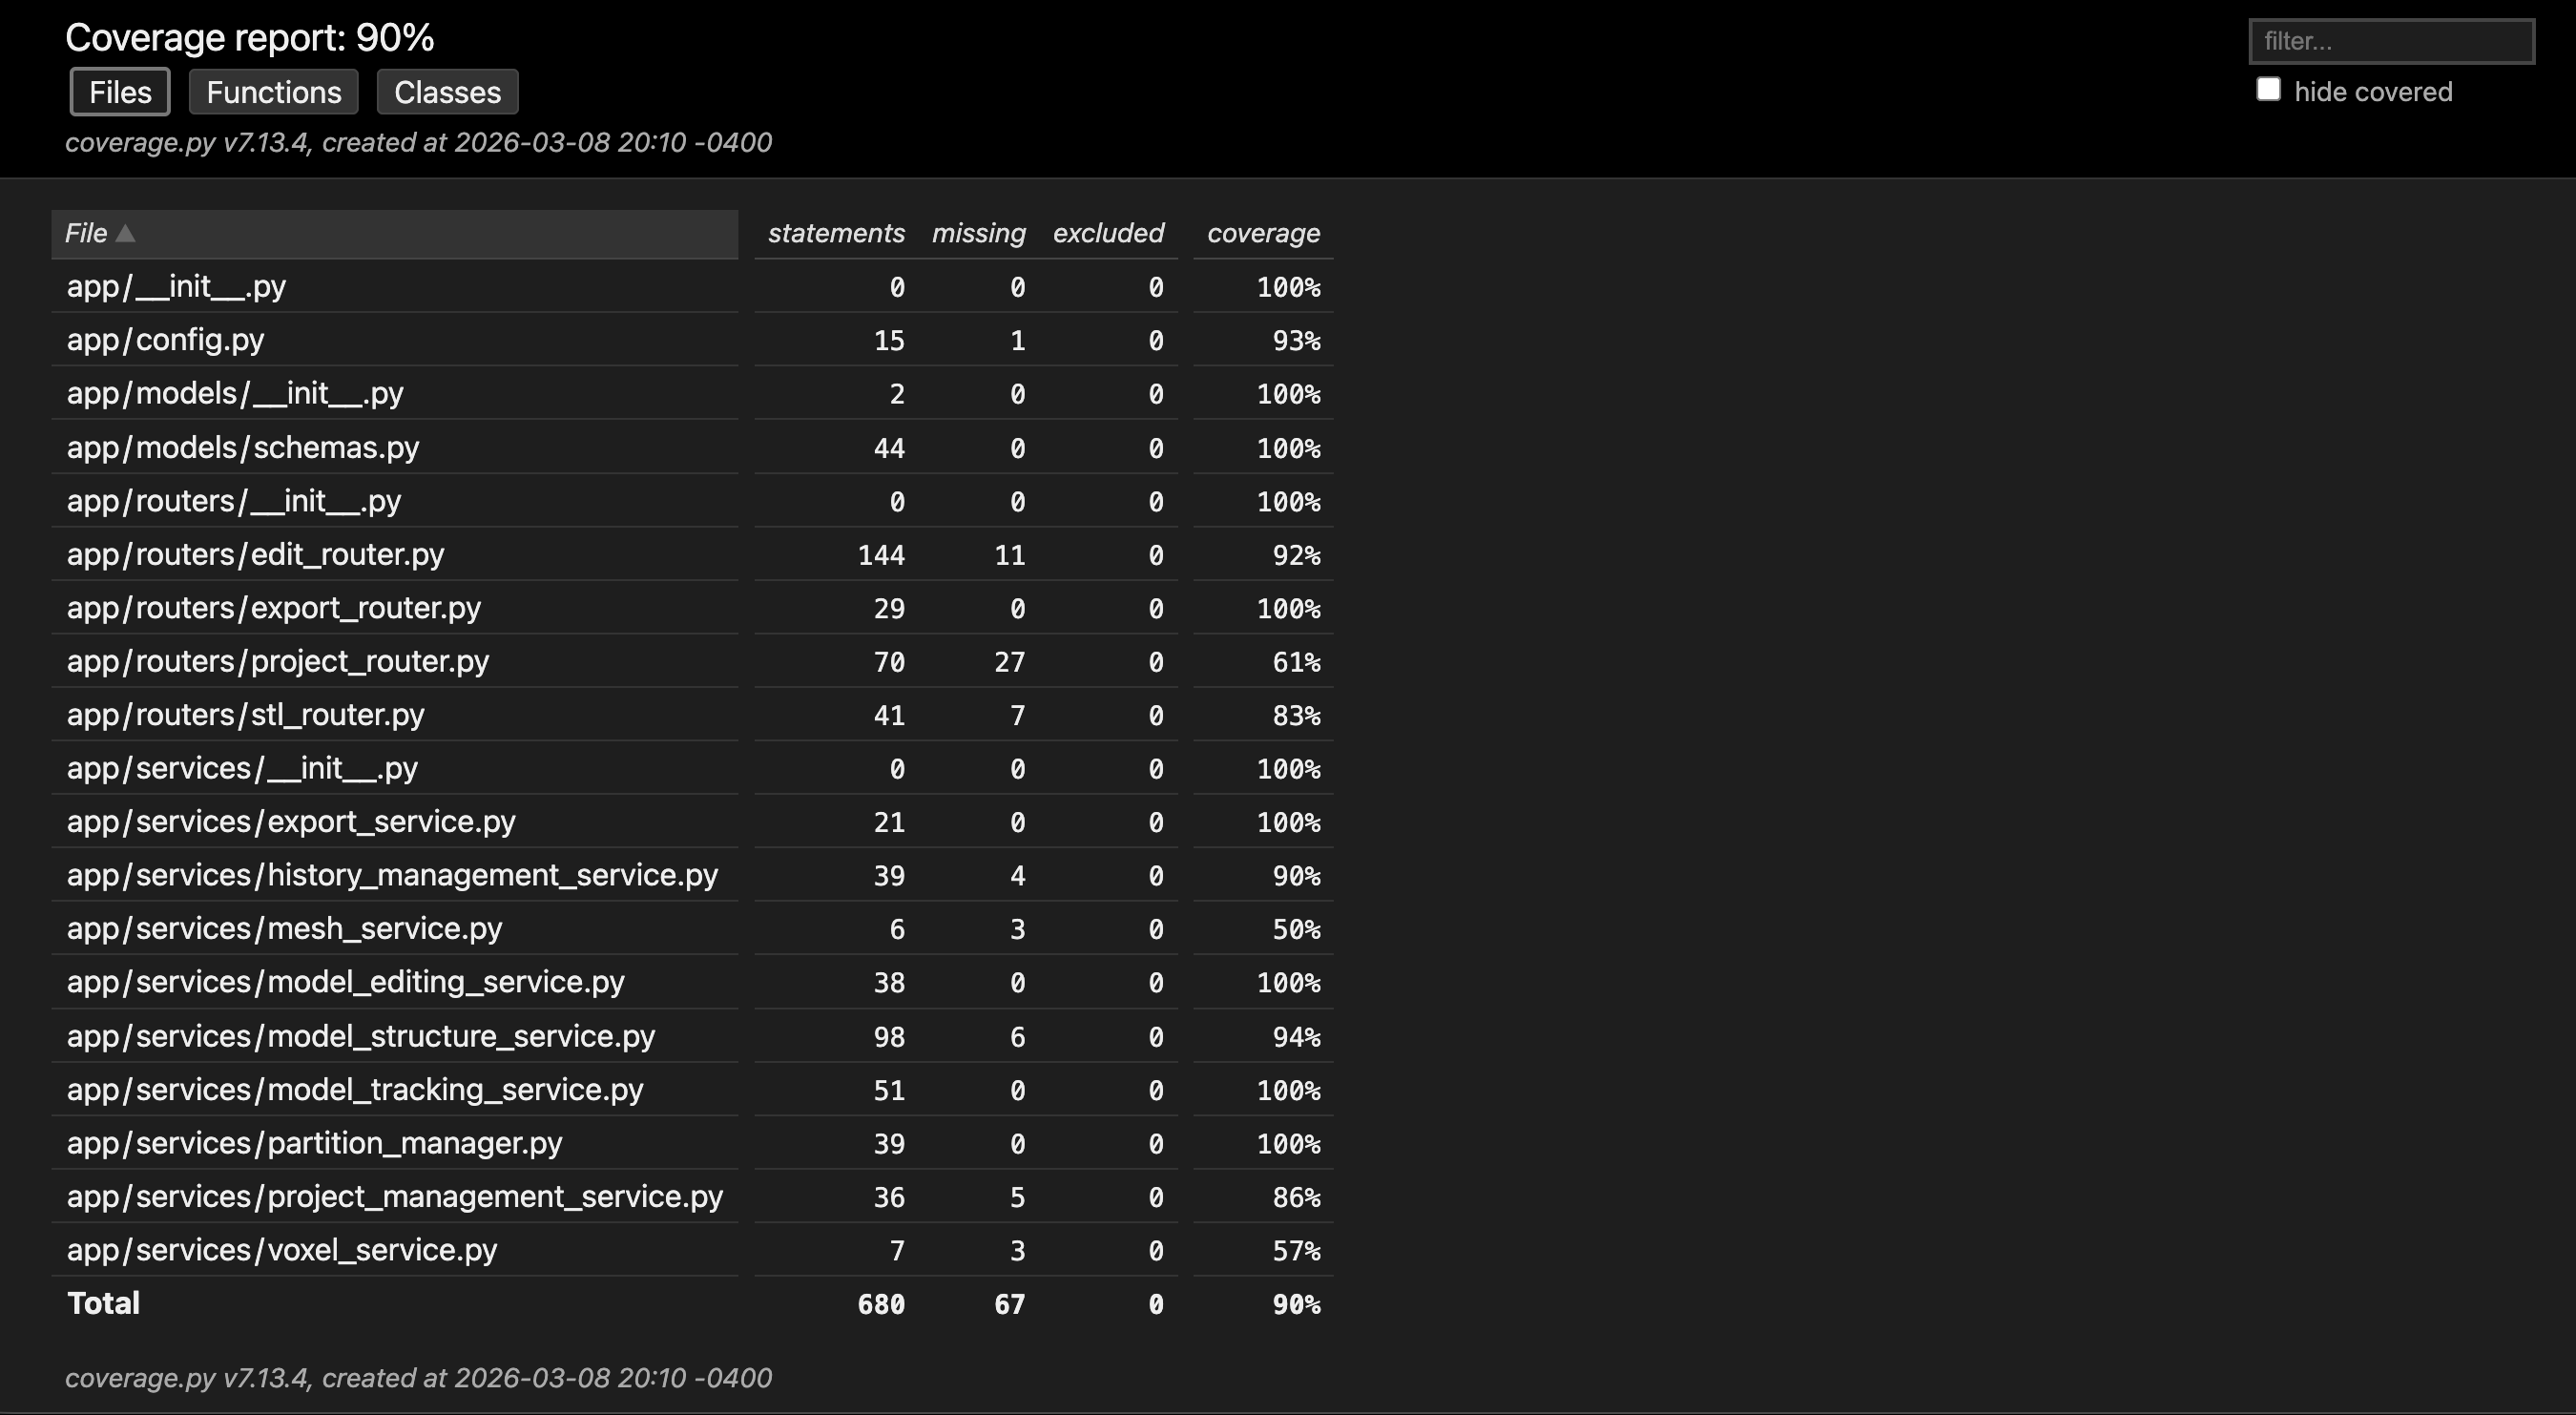
\includegraphics[width=\textwidth]{python-coverage.png}
\caption{Python Code Coverage}
\label{fig:python-coverage}
\end{figure}

The backend codebase has an overall code coverage of 90\% for statements, branches, functions, and lines. The code coverage overall met the VnV Plan's requirement of 50\%. The \texttt{voxel\_service.py} was the file that was the most difficult to test because it utilizes the \texttt{trimesh} library for voxelization. The team will furthur analyze the code coverage of the \texttt{voxel\_service.py} file to understand which parts of the code are not being tested and improve the coverage of the file.


\subsection{TypeScript Code Coverage}

The following section analyzes the code coverage of the TypeScript code in the frontend. The analysis is provided in the Figure~\ref{fig:typescript-coverage} and is a measure of how much of the code is being tested, and helps us understand which parts of the code are not being tested.

\begin{figure}[H]
\centering
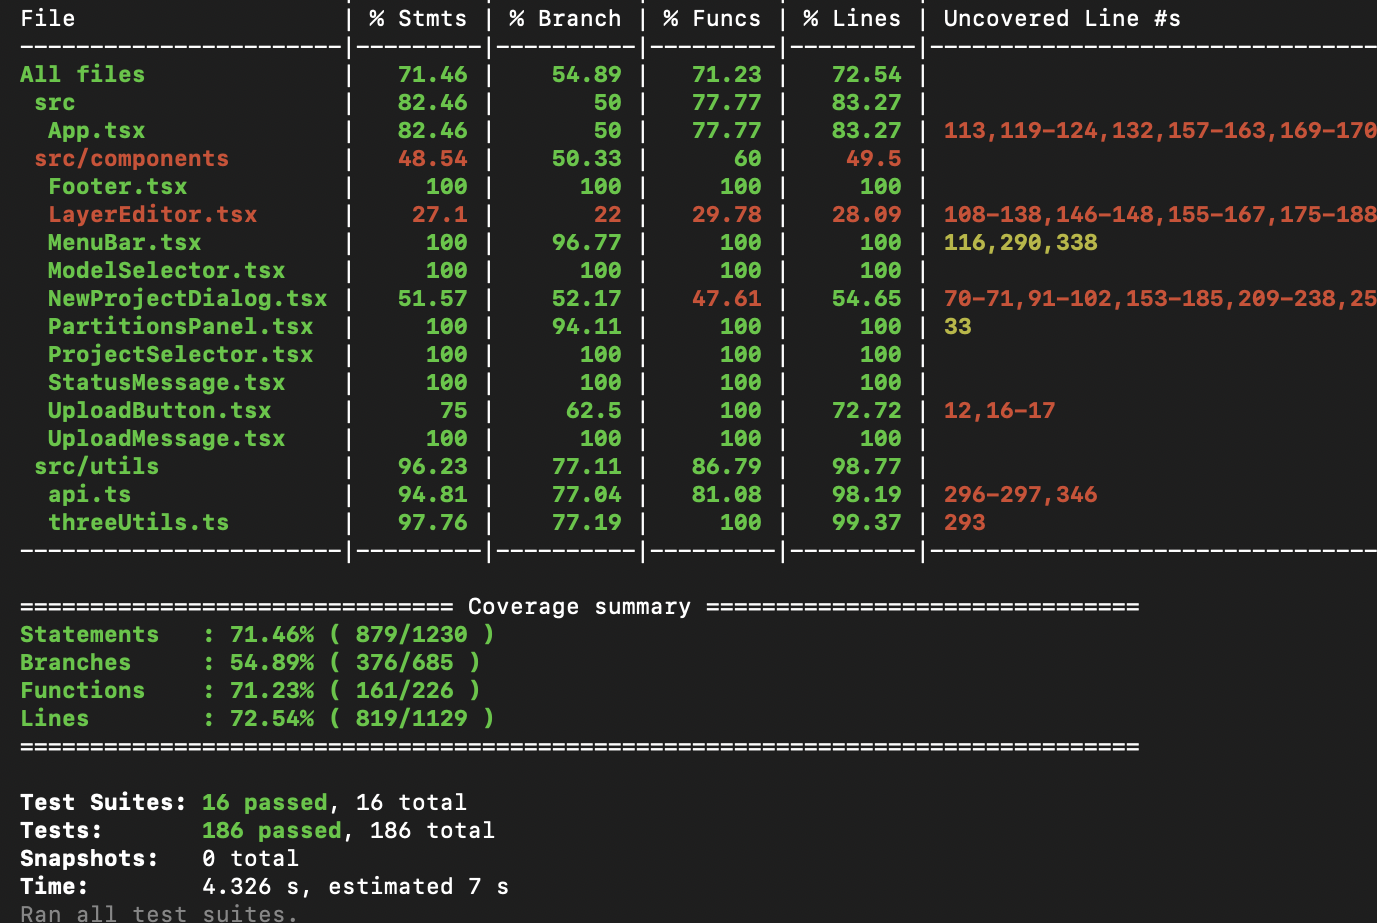
\includegraphics[width=\textwidth]{typescript-coverage.png}
\caption{TypeScript Code Coverage}
\label{fig:typescript-coverage}
\end{figure}

The frontend codebase has an overall code coverage of 83.08\% for statements, 65.98\% for branches, 85.39\% for functions, and 84.14\% for lines. The code coverage overall met the VnV Plan's requirement of 50\%. The team will continue to improve the coverage of the frontend codebase in the future.
\bibliographystyle{plainnat}
\bibliography{../../refs/References}

\newpage{}
\section*{Appendix --- Reflection}

The information in this section will be used to evaluate the team members on the
graduate attribute of Reflection.

\input{../Reflection.tex}

% \begin{enumerate}
%   \item What went well while writing this deliverable? 
%   \item What pain points did you experience during this deliverable, and how
%     did you resolve them?
%   \item Which parts of this document stemmed from speaking to your client(s) or
%   a proxy (e.g. your peers)? Which ones were not, and why?
%   \item In what ways was the Verification and Validation (VnV) Plan different
%   from the activities that were actually conducted for VnV?  If there were
%   differences, what changes required the modification in the plan?  Why did
%   these changes occur?  Would you be able to anticipate these changes in future
%   projects?  If there weren't any differences, how was your team able to clearly
%   predict a feasible amount of effort and the right tasks needed to build the
%   evidence that demonstrates the required quality?  (It is expected that most
%   teams will have had to deviate from their original VnV Plan.)
% \end{enumerate}

\subsubsection*{1. What went well while writing this deliverable?}
\bigskip\bigskip
\textbf{Omar: } The main thing that went well was connecting the VnV plan with the VnV report. The plan already defined the tests clearly, so it was straightforward to structure the report around usability, performance, compliance, maintainability, and security. The usability testing also went well since we were able to get feedback from both technical and non-technical users, which helped validate that the interface and main features were intuitive.
\newline
\newline
\textbf{Daniel: } I worked on the backend unit tests, as well as the organization of the usability test with our supervisor and her graduate students, which both went fairly smoothly in spite of the time crunch. The reorganization of the backend into cohesive modules and functions that I participated in was extremely helpful when generating all unit test cases, as well as their relative simplicity. The structure of the usability test - providing as little instruction as possible - also made it easy to identify parts of the software that still need work in terms of understandability.
\newline
\newline
\textbf{Andrew: } I worked on UI unit tests, listing all functional requirements in the report, and explaining the alternative COMSOL to AutoVox. Writing the UI tests went well, and I learned a lot about mocking modules, and making sure functions that needed to be fired and validated helped find any errors in the codebase.
\newline
\newline
\textbf{Olivia: } During this deliverable, I helped write some of the backend unit tests and was the primary person writing the usability report after usability testing, which was conducted by all group members. Due to the nature of this deliverable, I think that it really helped us narrow down some of the major areas that require improvement and further development as well as build confidence in the code that was already developed. With the final deadlines quickly approaching, there is a lot to do in very little time. Therefore, this type of direction is important to ensure that we make the best use out of the time we have remaining. 
\newline
\newline
\textbf{Khalid: } I worked on the unit tests and traceability between the test cases and the requirements. Having the traceability between the functional requirements and modules in the MIS document was very helpful in ensuring that all the test cases were covered and that the test cases were testing the correct functionality. It was also helpful to have the traceability between the test cases and the modules in the VnV Plan document. Overall, this deliverable went really well as everything was clearly defined and we were able to complete it on time. Another thing that was helpful was the fact that I didn't have much university work to do at the same time, so I was able to focus on this deliverable and get it done on time.

\subsubsection*{2. What pain points did you experience during this deliverable, and how
did you resolve them?}
\bigskip
\textbf{Omar: } One difficulty was making sure the report matched the VnV plan without repeating the same information. Since the plan already explains how tests are performed, the report had to focus more on results and evaluation. Another challenge was presenting the nonfunctional testing clearly, especially performance results, which required organizing the data into tables and graphs. Following the structure of the reference VnV report helped resolve this.
\newline
\newline
\textbf{Daniel: } Less of a pain point and more a frustration due to lack of experience; when generating unit tests my primary struggle was learning proper use of pytest and mocking classes, as well as when to mock. While I had planned to become familiar with it prior to needing to write these tests, other commitments prevented me from doing so, and I had to learn on the fly how to accomplish what I wanted to do. Fortunately, it was less complex once I figured out the syntax and I was able to finish all unit tests by the deadline I promised.
\newline
\newline
\textbf{Andrew: } I didn't experience many pain points, however it was hard to see exactly what our report should look like. The rubric wasn't that detailed, and the only way to see what to do correctly was to check prior submissions on the GitLab.
\newline
\newline
\textbf{Olivia: } In relation to the usability testing, one of the challenges that we experienced was choosing exactly how much guidance to give the user as they interacted with the software. We want to be able to provide enough structure and context so that the user is able to understand what we want them to do and how they can do it, while not making instructions too explicit in a way that compromises how a user would intuitively interact with and navigate through the software. While we went into the usability testing with a plan, things were definitely adapted in the moment. I think this is a natural part of usability testing. While you can have an idea on how you think people will interact with something, reality isn’t always what you imagine. If we decide to conduct another round of usability testing within the coming weeks after further developing the software, there will definitely be changes in the structure and method we choose to conduct usability testing that reflect some of our observations during the first round.
\newline
\newline
\textbf{Khalid: } I didn't experience much pain points during this deliverable. The only pain point I had was just the amount of repetitive work that was required to document the test cases and the requirements. However, I was able to resolve it by breaking down the work into smaller tasks and completing them one by one.

\subsubsection*{3. Which parts of this document stemmed from speaking to your client(s) or
a proxy (e.g. your peers)? Which ones were not, and why?}
\bigskip
Several parts of this document came from discussions with our supervisor and with a proxy (our peers). The scope of \textbf{functional and non-functional testing}---what needed to be tested and how, was conducted by speaking to the proxy and jointly defining the test objectives and coverage. The \textbf{Comparison to Existing Implementation} section came from speaking to our supervisor and to the graduate students who use the lab's 3D printing workflow. Those conversations helped us understand how they currently complete their objectives (e.g., with COMSOL) and what AutoVox should improve or replace. \textbf{Unit testing}, \textbf{automated testing}, and \textbf{coverage} were driven mainly by the proxy, we relied on peer discussion and shared standards to decide frameworks (e.g., PyTest, Jest), what to automate, and what coverage targets to aim for. \textbf{Changes due to testing} came from a mix of both: the proxy helped prioritize and validate technical changes, while the supervisor and graduate students provided context on whether those changes aligned with real usage and research needs.

\subsubsection*{4. In what ways was the Verification and Validation (VnV) Plan different from the activities that were actually conducted for VnV?  If there were 
differences, what changes required the modification in the plan?  Why did these changes occur?  Would you be able to anticipate these changes in future 
projects?  If there weren't any differences, how was your team able to clearly predict a feasible amount of effort and the right tasks needed to build the 
evidence that demonstrates the required quality?  (It is expected that most teams will have had to deviate from their original VnV Plan.)}
We did not make any major changes to the VnV Plan, the activities we conducted aligned with what was planned. We were able to predict a feasible amount of effort and the right tasks mainly because the plan was well scoped and supported by strong traceability. The traceability between the functional requirements (SRS), the modules (MIS and Module Guide), and the test cases in the VnV Plan made it clear which tests were needed and what they had to cover, so we could estimate effort and avoid gaps or duplicate work. The backend had also been reorganized into cohesive modules and functions before we wrote the unit tests, which made the test cases straightforward to implement and kept the workload manageable. For usability testing, the plan specified the overall approach (e.g., exploratory testing with minimal instruction and a task-based evaluation) but left out the exact list of tasks. When we ran the usability test, we did refine the specific tasks and the level of guidance given to participants (e.g. how much context to provide before each task). These were minor adjustments rather than changes to the plan itself, and they did not affect the planned objectives or deliverables. In future projects, we would again rely on clear traceability and a plan that fixes the strategy and scope while allowing small operational details (like concrete usability tasks) to be finalized at execution time.

\end{document}
